%% =====================================================================
%% HICA-S -- manuscript for Computers & Operations Research
%% Source of all numbers: HICA-S_Master_Writeup.md (rev. 2, 2026-09-28).
%% Lines marked "% VERIFY" must be checked against the primary source
%% before submission (bibliographic metadata or a literature claim).
%% Lines marked "% TODO" need input from the author.
%% Revision (2026-09-30): novelty claim rewritten around Sol (1994);
%% decomposition order set fixed; Thm (price of locality) example numbers
%% fixed; abstract instance counts fixed; several wording fixes.
%% =====================================================================
\documentclass[review,12pt]{elsarticle}

\usepackage{amsmath,amssymb,amsthm}
\usepackage{booktabs}
\usepackage{threeparttable}
\usepackage{array}
\usepackage{multirow}
\usepackage{graphicx}
\usepackage{algorithm}
\usepackage{algpseudocode}
\usepackage{tikz}
\usetikzlibrary{arrows.meta,positioning,fit,backgrounds}
\usepackage[hidelinks]{hyperref}
% Pseudocode floats are called "Procedure" to avoid a clash with the names
% Algorithm A (route generation), B (winner determination), C (payments).
\floatname{algorithm}{Procedure}
\algrenewcommand\algorithmicrequire{\textbf{Input:}}
\algrenewcommand\algorithmicensure{\textbf{Output:}}

\newtheorem{theorem}{Theorem}
\newtheorem{lemma}[theorem]{Lemma}
\newtheorem{proposition}[theorem]{Proposition}
\newtheorem{corollary}[theorem]{Corollary}
\theoremstyle{definition}
\newtheorem{definition}[theorem]{Definition}
\newtheorem{assumption}{Assumption}
\renewcommand{\theassumption}{A\arabic{assumption}}
\newtheorem{example}[theorem]{Example}
\theoremstyle{remark}
\newtheorem{remark}[theorem]{Remark}

\newcommand{\Kstar}{\mathcal{K}^\star}
\newcommand{\lth}{\underline{\theta}}
\newcommand{\uth}{\overline{\theta}}
\newcommand{\R}{\mathbb{R}}
\newcommand{\FD}{\mathrm{FD}}

\journal{Computers \& Operations Research}
\bibliographystyle{elsarticle-harv}

\begin{document}

\begin{frontmatter}

\title{Truthful route-bundle procurement with gigworkers and occasional
drivers: the local pruning frontier of bid-independent route generation}

\author{Tran An Khoa}
\ead{} % TODO: e-mail
\address{International University, Vietnam National University Ho Chi Minh
City, Ho Chi Minh City, Vietnam} % TODO: add school/department

\begin{abstract}
A delivery platform that buys service from gigworkers, who drive open
routes, and occasional drivers, who detour from a personal trip, can make
truthful cost reporting a dominant strategy by solving the winner
determination problem and all Clarke-pivot counterfactuals exactly on a
route pool that is generated before any bid is observed. The size of that
pool is the practical bottleneck: gigworkers have no detour budget to anchor
the search, and on five experimental instances only 0.4--1.5\% of the
generated routes are optimal for any of 1,000 sampled bid profiles. We
characterise exactly how far such a pool can be pruned by a rule that reads
neither bids nor other drivers' data. We define an envelope that completes
subset routes with a publicly priced fixed fleet, prove that deleting every
route outside the resulting \emph{local frontier} preserves the optimal
value, every removal value and all payments, and prove conversely that every
retained route is indispensable in some instance with the same local
information. We then construct instances in which a single gigworker's
frontier has $\Theta(n^B)$ routes, none ever optimal, so the enumeration
bound is tight for the whole class of such rules. A provably safe label rule
reaches the frontier with 35--76\% fewer label extensions. In a
pre-registered computational study, the frontier removes 75--100\% of the
pool without changing any payment, and joint bidding, endogenous bundling
and truthful payments matter only where the crowd competes with the fixed
fleet: there, they account for 5.8\%, 11.3\% and a 14.1\% payout premium,
respectively.
\end{abstract}

\begin{keyword}
Crowdshipping \sep Mechanism design \sep VCG auction \sep
Pickup and delivery \sep Column pruning \sep Occasional drivers
\end{keyword}

\end{frontmatter}

%% Highlights (submit as a separate file, max. 85 characters each):
%% - Exact VCG procurement from gigworkers and occasional drivers
%% - The local pruning frontier: smallest safe bid-independent route pool
%% - Tightness: frontier can hold Theta(n^B) routes that are never optimal
%% - A waiting-aware label rule reaches the frontier with far less work
%% - Crowd value appears only where it can compete with the fixed fleet

% =====================================================================
\section{Introduction}
\label{sec:intro}
% =====================================================================

Last-mile delivery platforms increasingly combine three sources of
capacity: a fixed-capacity fleet operated under contract, gigworkers who
accept multi-stop routes through an application, and occasional drivers
who carry parcels along a trip they would make anyway
\citep{archetti2016vrpod,luy2024workforce}. The first source has a known
price. The other two do not: a driver's value of time is private, and a
platform that pays what drivers claim invites them to overstate it. The
standard remedy is a Vickrey--Clarke--Groves (VCG) mechanism, which selects
the cost-minimising allocation and pays each winner her externality on the
others; truthful reporting then becomes a dominant strategy
\citep{nisan2007agt}. In routing applications the mechanism is implemented
by letting the platform generate candidate routes, collecting one scalar
bid per driver, solving a set-partitioning winner-determination problem,
and re-solving it once per winner to compute the Clarke-pivot payments
\citep{zou2022mechanisms,li2026auction}.

For this construction to remain truthful, the route pool must be fixed
before any bid is seen. The mechanism is then VCG on a bid-independent
range, and dominant-strategy incentive compatibility follows from the
maximal-in-range argument \citep{nisan2007computationally}. The price of
this requirement is the size of the pool. For an occasional driver, the
detour budget anchors the search: adding orders can only lengthen the
detour, so infeasible bundles and all their supersets can be discarded
early \citep{li2026auction}. A gigworker has no such anchor. Her route is
open, only time windows limit it, and feasibility is not monotone in the
bundle, so the pool grows as $\Theta(n^B)$ in the number of orders $n$ for
a bundle cap $B$. On our experimental instances, occasional drivers' pools
are only 0.7--1.7\% of gigworkers' pools, and on five of them only
0.4--1.5\% of all generated routes are optimal for any of 1,000 sampled bid
profiles. Every cheap rule we tried for removing the remaining routes either
deleted routes that some bid profile needs, or pruned almost nothing.

This paper asks, and answers, the question behind that experience: how far
can a route pool be pruned, before bids are observed, by a rule that uses
only the pruned driver's own data? The question matters because any rule
that reads bids changes the allocation range and can destroy truthfulness,
and any rule that reasons about other drivers must solve a problem that is
itself NP-hard. The answer is an explicit object, the \emph{local
frontier}, together with a proof that it cannot be improved upon within
this class of rules and a construction showing how large it can be.

\paragraph{Contributions} The paper makes the following contributions.

\begin{enumerate}
\item \emph{The local pruning frontier} (Theorem~\ref{thm:frontier}). We
define an envelope that compares each route with the cheapest subset route
of the same driver whose unserved orders are sent to the fixed fleet,
uniformly over the admissible report range. Deleting every route outside
the resulting frontier $\Kstar_i$ preserves the optimal value of the
winner-determination problem, every removal value, and hence all VCG
payments. Conversely, every route in $\Kstar_i$ is indispensable in some
instance that is indistinguishable from the given one using the driver's
own data, so $\Kstar_i$ is the unique minimal pool retained by any
deterministic rule that reads only that data.
\item \emph{The price of locality} (Theorem~\ref{thm:pol}). We construct
Euclidean instances in which a single gigworker's frontier contains
$\sum_{k\le B}\binom nk=\Theta(n^B)$ routes, none of which is optimal for any
bid profile. The $O(n^B)$ enumeration bound is therefore tight for the
whole class of local bid-independent rules, and the gap between the two
driver classes is structural rather than a shortcoming of a particular
algorithm.
\item \emph{A provably safe label rule} (Theorems~\ref{thm:labelbound}
and~\ref{thm:preserve}). We move part of the frontier reasoning inside the
label-setting procedure by adapting rollback pruning
\citep{lozano2016exact}. Because working time is priced and waiting is
allowed, the direct adaptation is unsafe (Example~\ref{ex:rollback}); a
correction for waiting absorption makes it safe. The rule leaves the
frontier unchanged and reduces label extensions by 35--76\% on our
instances.
\item \emph{Payment decomposition with a matching negative result}
(Section~\ref{sec:payments}). With a separable outside option, the
counterfactual solves decompose along the components of a static conflict
graph; a shared capacity on the outside option breaks the decomposition.
We report that the decomposition brings little benefit on our instances,
because the conflict graph is almost always connected where the crowd is
competitive.
\item \emph{A pre-registered computational study} of five research
questions. All parameters were locked and hashed before the main runs.
The frontier removes 75--100\% of the pool without changing any payment,
and, in the regime dominated by the fixed fleet, certifies in advance that
60\% of the drivers with a feasible route need not take part in the
auction. The economic effects of joint bidding, endogenous bundling and
truthfulness are all governed by one condition: whether the crowd can
compete with the fixed fleet.
\end{enumerate}

We do not claim a new incentive-compatibility result: the mechanism is
exact VCG on a bid-independent range, and its truthfulness is classical.
Nor do we claim the driver taxonomy, which we adopt from
\citet{luy2024workforce}. Although the two strategic classes have
different route geometries, both have costs affine in one scalar report,
so the winner-determination problem cannot tell a gigworker's column from
an occasional driver's column; the classes differ in the distribution of
columns they generate, not in the structure of the mechanism. That
difference in column distributions is precisely what the local frontier
and the price of locality make precise.

\paragraph{Organisation} Section~\ref{sec:lit} reviews related work.
Section~\ref{sec:model} states the model and the mechanism.
Section~\ref{sec:algA} describes bid-independent route generation.
Section~\ref{sec:frontier} develops the local pruning frontier and the
price of locality, and Section~\ref{sec:label} the label rule.
Section~\ref{sec:payments} treats payment computation.
Section~\ref{sec:experiments} reports the computational study,
Section~\ref{sec:discussion} discusses implications and limitations, and
Section~\ref{sec:conclusion} concludes. Longer proofs are in
\ref{app:proofs}.

% =====================================================================
\section{Related literature}
\label{sec:lit}
% =====================================================================

\subsection{Crowdshipping, hybrid fleets and procurement mechanisms}

\citet{archetti2016vrpod} introduced occasional drivers into vehicle
routing, with compensation set by the company rather than elicited.
\citet{luy2024workforce} distinguish fixed drivers, gigworkers and
occasional drivers in strategic workforce planning, treating driver costs
as known inputs. Several papers elicit costs. \citet{triki2021combinatorial}
lets occasional drivers bid on bundles alongside a company fleet but
does not establish incentive compatibility.
\citet{mancini2022bundle} generate bundles for occasional drivers along
travel corridors without a private-cost mechanism. \citet{chen2023truthful}
obtain a truthful reverse auction for occasional couriers with bundles
selected by the couriers themselves, so bundle selection is outside the
incentive analysis. \citet{zou2022mechanisms} give an exact VCG mechanism
with Clarke-pivot payments on a platform-generated job pool, with a
non-strategic backup vehicle and depot-based jobs. \citet{oyama2025market}
study market-based matching with task bundling, using a truthful auction
inside a sub-problem and a fluid approximation at the master level.
\citet{xu2026incentive} design incentive-compatible auctions for a hybrid
fleet in which only the crowd bids. Closest to this paper,
\citet{li2026auction} generate a route pool by solving pickup-and-delivery
problems with recursive branching that exploits the spatial monotonicity
of detour time, run exact VCG on it, and propose a greedy second-best
mechanism with a regret bound; their crowd carriers form a single
detour-constrained class.

Table~\ref{tab:positioning} summarises these studies. None treats an
open-route class and a detour-constrained class as strategic bidders
within one truthful mechanism, and none characterises how far a
bid-independent pool can be reduced without affecting the VCG outcome.

\begin{table}[t]
\centering
\caption{Positioning against the closest related studies.}
\label{tab:positioning}
\footnotesize
\setlength{\tabcolsep}{3pt}
\begin{tabular}{p{2.6cm}p{1.7cm}p{1.9cm}p{1.8cm}p{2.1cm}p{1.9cm}p{1.8cm}}
\toprule
Study & Open-route class bids & Detour class bids & Outside option & Bundle source & Incentive property & Pool reduction characterised \\
\midrule
\citet{archetti2016vrpod} & Company fleet & No bidding & -- & -- & -- & No \\
\citet{triki2021combinatorial} & Company fleet & Yes & -- & Bids & Not shown & No \\
\citet{zou2022mechanisms} & No & Yes (depot-based) & Backup vehicle & Platform & Exact VCG & No \\
\citet{mancini2022bundle} & No & -- & -- & Corridors & -- & No \\
\citet{chen2023truthful} & No & Yes & -- & Couriers & DSIC, fixed bundle & No \\
\citet{luy2024workforce} & Known cost & Known cost & Fixed drivers & -- & -- & No \\
\citet{oyama2025market} & One population & -- & Opt-out & Task chains & Truthful sub-auction & No \\
\citet{xu2026incentive} & Non-strategic & Yes & Yes & Predetermined & Yes & No \\
\citet{li2026auction} & No & Yes & Fixed price & Platform & Exact VCG, greedy & Detour-monotone branching \\
This paper & Yes & Yes & Fixed price & Platform, bid-independent & Exact VCG & Frontier and tightness \\
\bottomrule
\end{tabular}
\end{table}
% VERIFY: each row against the primary source before submission.

\subsection{Safe reduction of column pools}

Deleting columns that cannot be needed is a classical preprocessing step.
In set covering, a column is dominated if a cheaper column covers a
superset of its rows \citep{beasley1987algorithm}; \citet{muller1998solving}
deletes a column when other columns partition it at lower total cost. Both
assume known costs and compare against the whole pool.
\citet{pereira2013robust} treat set-covering costs as intervals, but seek a
single min--max-regret solution rather than a deletion rule that is exact
for every cost realisation.

In column generation, \citet{vanderbeck1994thesis} calls a column dominated
if another column has no larger reduced cost for all values of the dual
variables within their domains, and undominated if, against every other
column, some dual vector gives it a strictly smaller reduced cost;
\citet{sol1994column} strengthens dominance to redundancy, in which a column
is replaced by a combination of its subcolumns of no smaller total cost
(both as summarised by \citealp[§5.1]{lubbecke2005selected}). The rule of
\citet{muller1998solving} is the fixed-cost, whole-pool analogue of
redundancy for set partitioning. Our frontier is a form of Sol's redundancy
in which the substitute consists of exactly one subroute of the same driver
together with outside-option columns. The restriction matters: Sol shows
that no column is redundant when all subproblems differ from one another,
and in our setting every driver is a distinct subproblem. It is the publicly
priced outside option, whose columns belong to no driver's convexity row,
that restores redundancy. In dual terms the outside option imposes the
inequalities $\pi_o\le q_o$, in the spirit of the dual-optimal inequalities
of \citet{valerio2005extra} and \citet{benamor2006dual}
(Remark~\ref{rem:lp}). Three features have no counterpart in these sources.
First, costs depend on a report ranging over a domain fixed by the mechanism
designer, and the substitute may vary with the report: a route is deleted if
for every admissible report some substitute is at least as cheap, which is
weaker than requiring a single substitute that is cheaper for all reports.
Second, safety is required for the integer optimum and for every
Clarke-pivot removal problem, not for pricing a linear relaxation. Third,
beyond the pairwise notion of an undominated column, we show that every
retained route is indispensable in some instance with the same local
information, so the frontier is minimal over all local bid-independent
rules, and that it can nonetheless have size $\Theta(n^B)$.
% VERIFY: Sol's statement about distinct subproblems is read from
% Lubbecke & Desrosiers (2005, p. 1015); check Sol (1994) itself.

On the mechanism side, \citet{aggarwal2006knapsack} and
\citet{kempe2010frugal} prune agents before running a VCG-type mechanism in
order to bound its frugality ratio; their pruning may depend on bids and is
not required to preserve the optimal value exactly.

\subsection{Label dominance and rollback pruning}

Algorithm~A uses forward label setting with the dominance rule of
\citet{dumas1991pickup}, in the form presented by
\citet{gschwind2018bidirectional}. Our label rule adapts rollback pruning
\citep{lozano2016exact}, which compares a partial path with the same path
skipping a node and relies on the dominance relation of
\citet{feillet2004exact}. In the elementary shortest path problem with
resource constraints, time is a resource and arriving earlier never costs
anything; in our cost model working time is priced and waiting is allowed,
which is why a correction is needed.

\subsection{Computing VCG payments}

Exact VCG payments require the winner-determination problem to be solved
once with and once without each winner, which \citet{nisan2000computationally}
identified as a central obstacle to deploying VCG in practice. For
shortest-path auctions, \citet{hershberger2001vickrey} show that all
payments can be obtained far faster than by independent re-solves.
% VERIFY: exact statement of Hershberger & Suri (2001) (undirected graphs,
% time of a single shortest-path computation); do NOT attribute the
% sqrt(n) bound to this paper -- that is Hershberger, Suri & Bhosle (2007).
\citet{bleischwitz2005accelerating} share bounds across the simultaneous
searches of a combinatorial auction; \citet{sandholm2005cabob} decompose a
single winner-determination solve along the components of a bid-conflict
graph; and \citet{bunz2015faster} prove a separability result for
core-constraint generation based on a bipartite conflict graph rebuilt at
every iteration. \citet{wilkens2012single} and \citet{li2026auction} avoid
the repeated solves altogether by relaxing exactness, at the cost of
truthfulness only in expectation or of an approximate allocation. Our
decomposition in Section~\ref{sec:payments} uses a unipartite conflict
graph that is built once from the pool and reused for all counterfactuals.

% =====================================================================
\section{Model and mechanism}
\label{sec:model}
% =====================================================================

\subsection{Orders, drivers and the fixed fleet}

A dispatch session is static and deterministic. It consists of a finite set
of orders $O$ and a set of strategic drivers $N=G\cup C$, where $G$ is the
set of gigworkers and $C$ the set of occasional drivers. Order $o\in O$ has
a pickup node $p_o$, a delivery node $d_o$, a demand, a release time, and
time windows at both nodes; an arrival before the opening of a window is
met by waiting. Travel distances $d(\cdot,\cdot)$ and times
$\tau(\cdot,\cdot)$ are nonnegative and satisfy the triangle inequality,
and service times are nonnegative. Every order can be delegated to the
fixed-capacity fleet (FD) at a public price $q_o\ge 0$; for $A\subseteq O$
we write $q(A)=\sum_{o\in A}q_o$. The platform publishes a bundle cap $B$.

A gigworker has a start location, an availability interval and a capacity;
her route is open and ends at its last delivery. An occasional driver has an
origin, a personal destination, a direct trip from one to the other, a
detour budget $\tau_i$, an availability interval and a capacity; her route
ends at the destination and its detour time may not exceed $\tau_i$. These
data are public or committed before the session opens
(Section~\ref{sec:discussion} discusses this assumption). A route $r$ of
driver $i$ serves a bundle $S_r\subseteq O$ with $1\le|S_r|\le B$ and is
feasible if pickups precede deliveries, every order has been released when
it is picked up, all time windows, the availability interval and the
capacity are respected, and, for an occasional driver, the route ends at
the destination within the detour budget.

\subsection{Costs}

Serving route $r$ costs driver $i$
\begin{equation}
  C_{ir}(\theta_i)=K_{ir}+\theta_i\,W_{ir},
  \label{eq:cost}
\end{equation}
where $K_{ir}\ge 0$ is a distance cost, $W_{ir}\ge 0$ is working time in
hours, and $\theta_i>0$ is the driver's private value of time. Both
coefficients are computed by the platform from public data. For a gigworker
with distance coefficient $\kappa_i$ and departure time $t_0$,
$K_{ir}=\kappa_i\cdot(\text{route length})$ and
$W_{ir}=(\text{completion time}-t_0)/60$, with times in minutes. For an
occasional driver, costs are incremental over the direct trip:
$K_{ir}=\kappa_i\max\{0,\text{route length}-\text{direct length}\}$ and
$W_{ir}=\max\{0,\text{route time}-\text{direct time}\}/60$. A driver who
reports $b_i$ in place of $\theta_i$ is evaluated at the reported cost
$c_{ir}(b_i)=K_{ir}+b_i W_{ir}$. The idle option of driver $i$ is the empty
route $0_i$ with $S_{0_i}=\emptyset$ and $K=W=0$.

The single-parameter form~\eqref{eq:cost} is an empirical approximation,
not merely a convenience. In last-mile geometry route time is close to
route length divided by speed plus service time, so the vectors
(length, time) of a driver's bundle menu lie close to one ray. In
preliminary measurements on instances of the same generator, the angular
spread of a driver's menu was about one degree, the median number of
distinct bundle orderings over the type range was one under tight time
windows, and the welfare loss from projecting a two-dimensional
(per-kilometre, per-hour) cost onto one parameter was 0.002--0.05\%. The
conclusion was unchanged when the variability of speed was inflated
eightfold: a change of speed rotates a driver's menu rather than spreading
it, and the spread is governed by the ratio of service time to route
length.
% TODO: report the setup of these measurements (instances, speed model,
% projection method) in a short appendix with one figure, or cite the thesis.

\subsection{Winner determination and payments}

Let $R_i$ be the route pool of driver $i$, fixed before bids are
collected. Given a report profile $b$, the winner-determination problem
(Algorithm~B) is
\begin{align}
V(R;b)=\min_{x,z}\;&\sum_{i\in N}\sum_{r\in R_i}c_{ir}(b_i)\,x_{ir}+\sum_{o\in O}q_o z_o
\label{eq:wdp}\\
\text{s.t.}\;&\sum_{i\in N}\sum_{r\in R_i:\,o\in S_r}x_{ir}+z_o=1 && o\in O,\notag\\
&\sum_{r\in R_i}x_{ir}\le 1 && i\in N,\notag\\
&x_{ir},z_o\in\{0,1\},\notag
\end{align}
where $x_{ir}=1$ if driver $i$ receives route $r$ and $z_o=1$ if order $o$
is delegated to FD. Every order is served exactly once, every driver
receives at most one route, and the problem is always feasible because FD
is uncapacitated. Ties are broken deterministically and independently of
reports: among optimal solutions we minimise the number of orders sent to
FD and then choose lexicographically by route identifier. $V_{-k}(R;b)$
denotes the optimal value of~\eqref{eq:wdp} with driver $k$ removed.
Algorithm~C pays each winner $i$ with selected route $r_i^\ast$
\begin{equation}
p_i=c_{ir_i^\ast}(b_i)+V_{-i}(R;b)-V(R;b),
\label{eq:payment}
\end{equation}
and pays losers nothing. Only solutions proven optimal with zero gap are
used.

\begin{proposition}[Truthfulness; adapted from the Groves--VCG argument]
\label{prop:dsic}
If the pools $R_i$ are fixed before reports are observed, every base and
removal problem is solved exactly with report-independent tie-breaking, and
each report is a nonnegative scalar entering the objective as in
\eqref{eq:wdp}, then truthful reporting is a dominant strategy for every
driver and every winner's utility is nonnegative.
\end{proposition}

This is the standard maximal-in-range argument
\citep{nisan2007computationally}; its proof does not depend on whether a
route belongs to a gigworker or an occasional driver, and we do not claim
it as a contribution.

\subsection{Report domain}
\label{sec:reportdomain}

The mechanism above places no restriction on reports. The pruning results
of Sections~\ref{sec:frontier} and~\ref{sec:label} are stated for a report
domain $\Theta=[\lth,\uth]$ with $0\le\lth<\uth$, announced before bidding;
pruning is exact for every report profile in $\Theta^N$. When pruning is
used, the message space is therefore restricted to $\Theta$. Setting
$\Theta=[0,\infty)$ removes the restriction at the price of a larger
frontier (Remark~\ref{rem:monotone}). In our experiments $\Theta=[18,25]$,
which coincides with the support of the baseline type distribution.

\subsection{Overview of the procedure}
\label{sec:overview}

Figure~\ref{fig:pipeline} and Procedure~\ref{alg:mechanism} summarise how
the components developed in the remainder of the paper fit together.
Everything to the left of the report collection step uses public data only;
this is what makes the allocation range independent of the reports.

\begin{figure}[t]
\centering
\resizebox{\textwidth}{!}{%
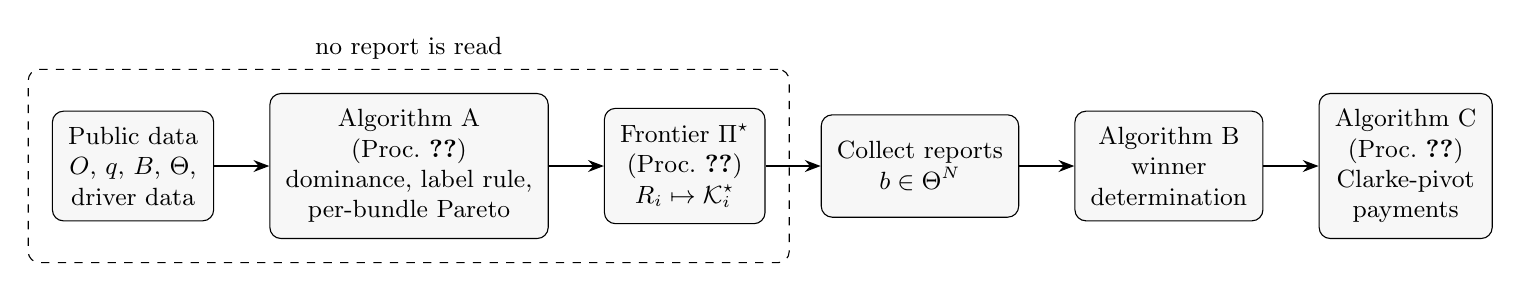
\begin{tikzpicture}[
  node distance=5mm and 7mm,
  every node/.style={font=\small},
  box/.style={rectangle, rounded corners, draw, align=center, minimum height=13mm, inner sep=2mm, fill=gray!6},
  arr/.style={-{Stealth[length=2mm]}, thick}]
\node[box] (data) {Public data\\$O$, $q$, $B$, $\Theta$,\\driver data};
\node[box, right=of data] (A) {Algorithm A\\(Proc.~\ref{alg:routegen})\\dominance, label rule,\\per-bundle Pareto};
\node[box, right=of A] (K) {Frontier $\Pi^\star$\\(Proc.~\ref{alg:frontier})\\$R_i\mapsto\Kstar_i$};
\node[box, right=of K] (bids) {Collect reports\\$b\in\Theta^N$};
\node[box, right=of bids] (B) {Algorithm B\\winner\\determination};
\node[box, right=of B] (C) {Algorithm C\\(Proc.~\ref{alg:payments})\\Clarke-pivot\\payments};
\draw[arr] (data) -- (A); \draw[arr] (A) -- (K); \draw[arr] (K) -- (bids);
\draw[arr] (bids) -- (B); \draw[arr] (B) -- (C);
\begin{scope}[on background layer]
\node[draw, dashed, rounded corners, inner sep=3mm, fit=(data)(A)(K),
      label={[font=\small]above:no report is read}] {};
\end{scope}
\end{tikzpicture}}
\caption{The procurement pipeline. Route generation and frontier pruning use
public data only and are completed before reports are collected; the pruned
pools define the allocation range on which exact VCG is run.}
\label{fig:pipeline}
\end{figure}

\begin{algorithm}[!htbp]
\caption{Truthful route-bundle procurement}
\label{alg:mechanism}
\begin{algorithmic}[1]
\Require orders $O$, FD prices $q$, bundle cap $B$, report domain $\Theta$, public driver data
\Ensure allocation $(x^\ast,z^\ast)$ and payments $(p_i)_{i\in N}$
\For{each driver $i\in N$} \Comment{no report is read in lines 1--4}
  \State $R_i\gets\textsc{GenerateRoutes}(i)$ \Comment{Algorithm A, Proc.~\ref{alg:routegen}}
  \State $R_i\gets\textsc{Frontier}(R_i,q,\Theta)$ \Comment{optional, Proc.~\ref{alg:frontier}}
\EndFor
\State publish a hash of $(R_i)_{i\in N}$; collect one report $b_i\in\Theta$ per driver
\State solve~\eqref{eq:wdp} on $R$ at $b$ to optimality $\to(x^\ast,z^\ast)$, $V(R;b)$ \Comment{Algorithm B}
\State $(p_i)_{i\in N}\gets\textsc{Payments}(R,b,x^\ast)$ \Comment{Algorithm C, Proc.~\ref{alg:payments}}
\State \Return $(x^\ast,z^\ast)$, $(p_i)_{i\in N}$
\end{algorithmic}
\end{algorithm}

% =====================================================================
\section{Bid-independent route generation}
\label{sec:algA}
% =====================================================================

Algorithm~A enumerates, for each driver separately, all feasible routes
with at most $B$ orders and keeps, for each bundle, the Pareto-minimal
pairs $(K,W)$. It never reads a report.

\paragraph{Labels} A label is a tuple $\ell=(v,IV,C,t,K,W)$ consisting of
the current node $v$, the set $IV$ of orders on board, the set $C$ of
delivered orders, the clock $t$ after service at $v$, and the accumulated
raw distance and time costs. A pickup of order $j$ is admissible if
$j\notin IV\cup C$, $|IV|+|C|<B$ and the pickup is reached before the
closing of its window; a delivery requires $j\in IV$; an occasional driver
may return to her destination once $IV=\emptyset$, provided the detour
budget is respected, and labels of an occasional driver that can no longer
reach the destination within the budget are discarded. Each transition waits
for the opening of the next window if necessary and advances the clock by
a nonnegative amount. A gigworker's label is complete when $IV=\emptyset$
and $C\neq\emptyset$; an occasional driver's label is complete when it has
reached the destination, after which the direct trip is subtracted once.
Labels are processed in rounds of increasing $|IV|+|C|$.

\paragraph{Dominance} Two labels are compared only if they share the key
$(v,IV,C)$; $\ell_A$ dominates $\ell_B$ if $t_A\le t_B$, $K_A\le K_B$ and
$W_A\le W_B$ with at least one strict inequality. This is the forward
dominance of \citet{dumas1991pickup}. The key cannot be coarsened in
general.

\begin{lemma}[Disjoint reachable completions]
\label{lem:disjoint}
Let $\ell_A$ and $\ell_B$ share $(v,IV)$ with $C_A\ne C_B$, and suppose some
$j\in C_B\setminus C_A$ has pickup closing time $l(p_j)<t_A$. Then every
completion of $\ell_B$ serves $j$ and no completion of $\ell_A$ does.
\end{lemma}

\begin{proof}
Delivered sets only grow along transitions, so every completion of
$\ell_B$ contains $j$. Since $j\notin IV$ (otherwise $j\in IV\cap C_B$) and
$j\notin C_A$, a completion of $\ell_A$ containing $j$ would pick $j$ up at
some time $t''\ge t_A>l(p_j)$, which is infeasible.
\end{proof}

Merging labels under the coarser key $(v,IV)$ can therefore discard the only
label able to reach some bundle. On 720 instances with $n\le 6$, both
coarsenings we tested (dropping $C$, or keeping only $|C|$) disagreed with
brute-force enumeration in 46--47\% of instances. A coarser key is safe for
a pair of labels only if $l(p_j)\ge\max\{t_A,t_B\}$ for every
$j\in C_A\triangle C_B$; this condition depends on both labels jointly and
cannot be encoded as a key computed per label.

Procedure~\ref{alg:routegen} states Algorithm~A in full. It contains three
pruning layers. Layer~1 is the label dominance above, applied within each
batch of labels that share the number of touched orders. Layer~2 keeps, for
each bundle, the Pareto-minimal pairs $(K,W)$ of the completed routes; it
never compares routes with different bundles, because the orders missing from
the smaller bundle would have to be served by someone. Layer~3 is the
optional FD-completion label rule of Section~\ref{sec:label}. Table~\ref{tab:layers}
contrasts the three layers with the frontier filter of
Section~\ref{sec:frontier}.

\begin{algorithm}[!htbp]
\caption{\textsc{GenerateRoutes}$(i)$: Algorithm A for one driver}
\label{alg:routegen}
\begin{algorithmic}[1]
\Require public data of driver $i$; orders $O$; cap $B$; flag \textit{useRule}
\Ensure route pool $R_i$ (Pareto-minimal $(K,W)$ per bundle)
\State $\mathcal L_0\gets\{(v_0,\emptyset,\emptyset,t_0,0,0)\}$; $\mathcal L_k\gets\emptyset$ for $k=1,\dots,B$; $\mathcal C\gets\emptyset$
\For{$k\gets 0$ \textbf{to} $B$} \Comment{$k=|IV|+|C|$, the number of touched orders}
  \State $\mathcal Q\gets\mathcal L_k$
  \While{$\mathcal Q\ne\emptyset$}
    \State $\mathcal Q\gets\textsc{FilterDominated}(\mathcal Q)$ \Comment{Layer 1: same key $(v,IV,C)$}
    \State $\mathcal Q'\gets\emptyset$
    \For{each label $\ell\in\mathcal Q$}
      \If{$i\in G$ \textbf{and} $IV(\ell)=\emptyset$ \textbf{and} $C(\ell)\ne\emptyset$}
        \State add $\ell$ to $\mathcal C$ \Comment{complete gigworker route; $\ell$ may still be extended}
      \EndIf
      \If{$i\in C$ \textbf{and} $IV(\ell)=\emptyset$ \textbf{and} $C(\ell)\ne\emptyset$}
        \State $\ell'\gets\textsc{TryHome}(\ell)$; \textbf{if} $\ell'\ne\bot$ \textbf{then} add $\ell'$ to $\mathcal C$ \Comment{checks the detour budget}
      \EndIf
      \For{each $j\in IV(\ell)$}
        \State $\ell'\gets\textsc{TryDelivery}(\ell,j)$
        \If{$\ell'\ne\bot$ \textbf{and not} (\textit{useRule} \textbf{and} $\textsc{RuleFires}(\ell')$)} add $\ell'$ to $\mathcal Q'$ \EndIf
      \EndFor
      \If{$k<B$}
        \For{each $j\in O\setminus(IV(\ell)\cup C(\ell))$}
          \State $\ell'\gets\textsc{TryPickup}(\ell,j)$
          \If{$\ell'\ne\bot$ \textbf{and not} (\textit{useRule} \textbf{and} $\textsc{RuleFires}(\ell')$)} add $\ell'$ to $\mathcal L_{k+1}$ \EndIf
        \EndFor
      \EndIf
    \EndFor
    \State $\mathcal Q\gets\mathcal Q'$ \Comment{each delivery adds one order to $C$}
  \EndWhile
\EndFor
\State for occasional drivers, subtract the direct trip from each complete label (Section~\ref{sec:model})
\For{each bundle $S$ appearing in $\mathcal C$}
  \State $R_i(S)\gets\textsc{ParetoFront}\bigl(\{(K_\ell,W_\ell):\ell\in\mathcal C,\ C(\ell)=S\}\bigr)$ \Comment{Layer 2}
\EndFor
\State \Return $R_i=\bigcup_S R_i(S)$, one route per distinct pair $(K,W)$
\end{algorithmic}
\end{algorithm}

\begin{table}[t]
\centering
\caption{Pruning layers of Algorithm A and the frontier filter.}
\label{tab:layers}
\small
\begin{tabular}{p{3.3cm}p{3.1cm}p{3.4cm}p{1.6cm}p{2.6cm}}
\toprule
Filter & Compares & Scope & Uses $q$? & When\\
\midrule
Layer 1: label dominance & label vs.\ label & same $(v,IV,C)$ & No & During generation\\
Layer 2: per-bundle Pareto & route vs.\ route & same bundle $S$ & No & After generation\\
Layer 3: label rule (Sec.~\ref{sec:label}) & partial route vs.\ FD, lower bound & any $T\subseteq P(L)$ & Yes & During generation\\
Frontier $\Pi^\star$ (Sec.~\ref{sec:frontier}) & route vs.\ subset route $+$ FD, exact & any $r'$ with $S_{r'}\subseteq S_r$ & Yes & After generation\\
\bottomrule
\end{tabular}
\end{table}

\paragraph{Properties} Algorithm~A is complete: for $n\le 6$ its output
coincides with brute-force enumeration. For fixed $B$ the pool of a driver
has size $O(|O|^B(2B)!/2^B)$. The pool, and a hash of it, are invariant
under any change of reports. Keeping only same-bundle Pareto-minimal pairs
is safe because $b\ge 0$.

\paragraph{The asymmetry between the classes} For an occasional driver the
detour budget provides a monotone bound: a lower bound on the detour of a
bundle eliminates the bundle and all its supersets before any sequence is
enumerated \citep{li2026auction}. For a gigworker the only constraints are
time windows. Two orders may each be servable while the pair is not, and a
bundle of distant orders remains feasible whenever the windows are wide, so
no bound as strong as a detour budget is available. On our instances the pool of
an occasional driver is 0.7--1.7\% of that of a gigworker.
Section~\ref{sec:frontier} shows that this asymmetry cannot be removed by
any local bid-independent pruning rule.

% =====================================================================
\section{The local pruning frontier}
\label{sec:frontier}
% =====================================================================

When the platform considers deleting a route $r$ of driver $i$ without
looking at the other drivers, the only substitutes it can certify are
those that involve nobody else: a route of the same driver that serves part
of $S_r$, with the remainder sent to FD. The frontier keeps exactly the
routes for which no such substitute is at least as cheap for every
admissible report. This section shows that deleting everything else is
safe, that nothing in the frontier can be deleted safely by any rule of
this kind, and that the frontier can nevertheless be very large.

\subsection{Definitions}

\begin{definition}[Local view, local rule, safety]
\label{def:local}
The local view of driver $i$ is $L_i=(O,q,B,\Theta,R_i)$. A local pruning
rule $\Pi$ is a deterministic map that assigns to every local view a set
$\Pi(L_i)\subseteq R_i$ of routes to delete; it is applied to every driver
and yields pools $R^\Pi_j=R_j\setminus\Pi(L_j)$. An instance is any finite
set of drivers whose pools consist of routes with bundles of size at most
$B$ and nonnegative coefficients. The rule is safe if $V(R^\Pi;b)=V(R;b)$
for every instance and every $b\in\Theta^N$.
\end{definition}

A local rule reads no report, so it leaves the allocation range fixed
before bidding and Proposition~\ref{prop:dsic} continues to apply to the
pruned mechanism.

\begin{definition}[FD-completion envelope and local frontier]
\label{def:frontier}
For $r\in R_i$ let $D(r)=\{r'\in R_i\cup\{0_i\}\setminus\{r\}:S_{r'}\subseteq S_r\}$
and
\[
E_r(b)=\min_{r'\in D(r)}\bigl\{c_{r'}(b)+q(S_r\setminus S_{r'})\bigr\},\qquad
\mu_r(b)=E_r(b)-c_r(b).
\]
The local frontier of driver $i$ is
$\Kstar_i=\{r\in R_i:\max_{b\in\Theta}\mu_r(b)>0\}$, and the rule $\Pi^\star$
deletes $R_i\setminus\Kstar_i$ for every driver.
\end{definition}

Because $0_i\in D(r)$, $E_r(b)\le q(S_r)$. The envelope $E_r$ is the
minimum of finitely many affine functions of $b$, hence concave and
piecewise linear, so $\mu_r$ is concave and its maximum over $\Theta$ is
attained at an endpoint or at a breakpoint of $E_r$. We use three
assumptions on the pool of the driver under study.

\begin{assumption}[No duplicates]\label{ass:nodup}
Distinct routes of $R_i$ with the same bundle have distinct pairs $(K,W)$.
\end{assumption}
\begin{assumption}[Downward closure]\label{ass:down}
For every $r'\in R_i$, every $T\subseteq S_{r'}$ and every $b\in\Theta$
there is $\hat r\in R_i\cup\{0_i\}$ with $S_{\hat r}=T$ and
$c_{\hat r}(b)\le c_{r'}(b)$.
\end{assumption}
\begin{assumption}[No free supersets]\label{ass:nofree}
If $r,r'\in R_i$ and $S_r\subsetneq S_{r'}$, then
$(K_r,W_r)\ne(K_{r'},W_{r'})$.
\end{assumption}

Assumption~\ref{ass:nofree} only excludes serving additional orders at
exactly zero additional distance and time. Assumptions~\ref{ass:nodup}
and~\ref{ass:down} are not additional modelling choices:

\begin{lemma}[Pools of Algorithm~A are downward closed]
\label{lem:downward}
Under the assumptions of Section~\ref{sec:model} (triangle inequality,
nonnegative service, lower time-window bounds met by waiting, upper bounds
on deadlines, availability, capacity and detour), every pool produced by
Algorithm~A without the label rule (\textit{useRule} false) satisfies
Assumptions~\ref{ass:nodup} and~\ref{ass:down}.
\end{lemma}

The distance part follows from the triangle inequality. The time part
requires a short induction over service start times, because a start time
is the maximum of the arrival time and the window opening, so arriving
earlier need not mean finishing earlier; the induction shows that removing
stops never delays any retained stop. The proof is in
\ref{app:downward}. Pools produced with the label rule need not be
downward closed; Theorem~\ref{thm:preserve} shows that this does not matter.

\subsection{An example}

The following example shows why a rule that sees only one driver cannot
delete routes that look useless for that driver.

\begin{example}[Twin instances]
\label{ex:twin}
Let gigworker $g$ face orders $o_1,o_2$ with $q_{o_1}=15$, $q_{o_2}=45$ and
$\Theta=[18,25]$, and own three routes: $r_a$ serving $\{o_1\}$ with
$(K,W)=(6,0.6)$; $r_b$ serving $\{o_2\}$ with $(8,0.8)$; and $r_c$ serving
$\{o_1,o_2\}$ with $(11,1.2)$. Route $r_a$ is outside the frontier, since
$E_{r_a}=q_{o_1}=15<6+0.6b$ on $\Theta$. Route $r_b$ is in the frontier,
since $E_{r_b}=45>8+0.8b$. Route $r_c$ is in the frontier, since
$E_{r_c}(18)=\min\{6+10.8+45,\;8+14.4+15,\;60\}=37.4>32.6=c_{r_c}(18)$. In
instance $I_0$, in which $g$ is the only driver, $r_c$ is optimal on all of
$\Theta$ and $r_b$ is never optimal. In instance $I_1$, which adds a driver
who serves $o_1$ at cost $0.5$, the optimum at $b=18$ is
$22.4+0.5=22.9$ and uses $r_b$; without $r_b$ it is $32.6$. A rule that
deletes $r_b$ --- for instance a per-driver hull across bundles, under which
$r_a$ dominates $r_b$ componentwise --- is correct on $I_0$ and wrong on
$I_1$, and no rule that sees only $g$'s data can tell the two instances
apart.
\end{example}

\subsection{Main result}

\begin{theorem}[Local pruning frontier]
\label{thm:frontier}
Let $\lth<\uth$.
\begin{enumerate}
\item[(a)] \emph{Safety.} If every pool satisfies
Assumption~\ref{ass:nodup}, then $\Pi^\star$ is safe. Moreover
$V_{-k}(R^{\Pi^\star};b)=V_{-k}(R;b)$ for every driver $k$ and every
$b\in\Theta^N$.
\item[(b)] \emph{Indispensability.} If $R_i$ satisfies
Assumptions~\ref{ass:nodup}--\ref{ass:nofree} and $r\in\Kstar_i$, there
exist an instance containing driver $i$ with the same local view $L_i$ and
a report profile $b\in\Theta^N$ such that every optimal allocation assigns
$r$ to $i$ and $V(R\setminus\{r\};b)\ge V(R;b)+\gamma/2$ for some
$\gamma>0$.
\item[(c)] \emph{Exactness.} Let $\Pi$ be any deterministic rule whose
output for driver $i$ depends only on $L_i$. If $\Pi$ is safe, then on local
views satisfying Assumptions~\ref{ass:nodup}--\ref{ass:nofree} it never
deletes a route of $\Kstar_i$. Hence $\Kstar_i$ is the unique minimal pool
retained by such rules, and $\Pi^\star$ attains it.
\end{enumerate}
\end{theorem}

The proof of part (a) rests on the fact that a deleted route can always be
replaced by a retained one, not merely by some route that may itself have
been deleted.

\begin{lemma}[A retained substitute exists]
\label{lem:substitute}
Let $R_i$ satisfy Assumption~\ref{ass:nodup} and $\lth<\uth$. For every
$r\in R_i\setminus\Kstar_i$ and every $b\in\Theta$ there is
$u\in\Kstar_i\cup\{0_i\}$ with $S_u\subseteq S_r$ and
$c_u(b)+q(S_r\setminus S_u)\le c_r(b)$.
\end{lemma}

\begin{proof}[Proof of Theorem~\ref{thm:frontier}(a)]
Fix an instance, a profile $b\in\Theta^N$ and an optimal allocation $\rho$
for the full pools. For every driver $j$ whose route $\rho_j$ is not in
$\Kstar_j\cup\{0_j\}$, Lemma~\ref{lem:substitute} gives
$u_j\in\Kstar_j\cup\{0_j\}$ with $S_{u_j}\subseteq S_{\rho_j}$ and
$c_{u_j}(b_j)+q(S_{\rho_j}\setminus S_{u_j})\le c_{\rho_j}(b_j)$. Replace
$\rho_j$ by $u_j$ and send $S_{\rho_j}\setminus S_{u_j}$ to FD. Bundles only
shrink, so they remain disjoint; every order is still served once; and no
other driver is affected, so all replacements can be made simultaneously.
The resulting allocation uses only pruned pools and costs at most
$V(R;b)$, so $V(R^{\Pi^\star};b)\le V(R;b)$; the reverse inequality holds
because pruned pools are subsets. Removing driver $k$ yields another
instance in which every remaining driver has the same local view, so the
same argument applies to $V_{-k}$.
\end{proof}

\begin{corollary}[VCG outcomes are preserved]
\label{cor:vcg}
Running Algorithms~B and~C on $R^{\Pi^\star}$ is VCG on a bid-independent
range and is therefore truthful and individually rational. At every
profile at which the full problem has a unique optimal allocation, the
pruned problem has the same allocation and every payment~\eqref{eq:payment}
coincides with its full-pool value.
\end{corollary}

\begin{proof}
The first statement is Proposition~\ref{prop:dsic}. Under uniqueness, any
pruned optimum has value $V(R;b)$ by Theorem~\ref{thm:frontier}(a) and is
feasible for the full pools, hence equal to the full optimum; $V$ and every
$V_{-k}$ coincide by part (a).
\end{proof}

Part (b) extends the local margin from subset routes to routes that overlap
$S_r$ arbitrarily.

\begin{lemma}[Margin against overlapping routes]
\label{lem:margin}
Let $R_i$ satisfy Assumptions~\ref{ass:down} and~\ref{ass:nofree},
$\lth<\uth$ and $r\in\Kstar_i$ with $S=S_r$. There are $b^\ast\in\Theta$ and
$\gamma>0$ such that
$c_{r'}(b^\ast)+q(S\setminus S_{r'})\ge c_r(b^\ast)+\gamma$ for every
$r'\in R_i\cup\{0_i\}\setminus\{r\}$.
\end{lemma}

\begin{proof}[Proof of Theorem~\ref{thm:frontier}(b)]
Let $b^\ast,\gamma$ be as in Lemma~\ref{lem:margin} and
$0<\varepsilon\le\gamma/(2B)$. The instance consists of driver $i$ with
report $b^\ast$ and, for every $x\in O\setminus S$, a driver $j_x$ whose pool
is a single route serving $\{x\}$ with $K=\varepsilon$ and $W=0$. The data
$O,q,B,\Theta,R_i$ are unchanged, so driver $i$ has local view $L_i$. Fix
the route $r'$ chosen for $i$. Orders in $S\setminus S_{r'}$ can only go to
FD; each $x\in O\setminus(S\cup S_{r'})$ is served at cost
$e_x=\min\{\varepsilon,q_x\}\le\varepsilon$. The best allocation given $r'$
therefore costs
$F(r')=c_{r'}(b^\ast)+q(S\setminus S_{r'})+\sum_{x\in O\setminus(S\cup S_{r'})}e_x$,
and by Lemma~\ref{lem:margin} and $|S_{r'}\setminus S|\le B$,
\[
F(r')-F(r)=c_{r'}(b^\ast)+q(S\setminus S_{r'})-c_r(b^\ast)-\sum_{x\in S_{r'}\setminus S}e_x\ge\gamma-B\varepsilon\ge\gamma/2 .
\]
Every optimal allocation therefore assigns $r$ to $i$, and removing $r$
raises the optimal value by at least $\gamma/2$.
\end{proof}

\begin{proof}[Proof of Theorem~\ref{thm:frontier}(c)]
Suppose $\Pi$ deletes some $r\in\Kstar_i$. In the instance of part (b),
driver $i$ has local view $L_i$, so $\Pi$ deletes $r$ there as well. Every
allocation in the pruned pools is an allocation in $R\setminus\{r\}$, hence
$V(R^\Pi;b)\ge V(R\setminus\{r\};b)>V(R;b)$ and $\Pi$ is not safe. Every
safe local rule thus deletes only routes outside $\Kstar_i$, and $\Pi^\star$
deletes all of them and is safe by part (a). A smallest element with respect
to inclusion is unique.
\end{proof}

Lemmas~\ref{lem:substitute} and~\ref{lem:margin} are proved in
\ref{app:proofs}.

\subsection{Scope of the result}

The minimality in Theorem~\ref{thm:frontier}(c) is relative to the class of
rules in Definition~\ref{def:local}, and it matters what lies outside it.

\begin{remark}[What the frontier is not]
\label{rem:scope}
The frontier can be beaten in three ways, each of which leaves the class of
Definition~\ref{def:local}. (i) \emph{Non-local rules} that use the public
data of other drivers remain bid-independent and preserve truthfulness. In
the instances of Theorem~\ref{thm:pol} below such a rule could delete every
route of the gigworker, but deciding this requires reasoning about the
other drivers' winner-determination problem, which is NP-hard for
$B\ge 3$ already at a single report profile: with one driver per 3-set,
each owning one route of cost zero, and $q_o=1$, the optimal value is zero
if and only if an exact cover by 3-sets exists. (ii) \emph{Instance-specific
rules}, which only need to be correct on the instance at hand, can retain
far less: on five experimental instances only 0.4--1.5\% of generated routes
are optimal for any of 1,000 sampled report profiles, whereas the frontier
retains 3--23\% of the pool on the same instances. (iii) \emph{Restricting
the class of instances} to geometrically realisable competitors weakens the
safety requirement; Remark~\ref{rem:realisable} bounds the effect.
\end{remark}

\begin{remark}[Realisability with genuine occasional drivers]
\label{rem:realisable}
The competitors $j_x$ in the proof of part (b) are abstract. They can be
replaced by occasional drivers whose origin and destination are the pickup
and delivery of $x$ and whose detour budget equals the total service time
$s_x$ at the two stops; under a general-position condition such a driver
can serve $x$ and nothing else, at a working-time cost of at least
$\lth s_x/60$ per order (1.20 with $s_x=4$ minutes and $\lth=18$). In a
synthetic audit, 556 of 563 frontier routes (98.8\%) remained indispensable
against such fully geometric competitors, and the prediction was never
violated. Whether a safe local rule can exploit this credit in general is
open: a gigworker route with waiting slack can absorb an extra order at
zero marginal cost.
\end{remark}

\begin{remark}[Monotonicity]
\label{rem:monotone}
$E_r$ is nondecreasing in every $q_o$, and the maximum of $\mu_r$ over a
larger interval is larger. The frontier therefore grows with the FD tariff
and with the width of $\Theta$: local pruning is strong when FD is cheap and
weak when it is expensive. With $\Theta=[0,\infty)$ the rule remains safe but
retains more routes.
\end{remark}

\begin{remark}[Computation]
\label{rem:computation}
$|D(r)|\le 2^Bf$, where $f$ bounds the number of routes per bundle. Since
$\mu_r$ is concave, membership in $\Kstar_i$ is decided by evaluating
$\mu_r$ at the endpoints of $\Theta$ and at the breakpoints of $E_r$, in
$O(|D(r)|\log|D(r)|)$ time; the whole frontier of a driver costs
$O(|R_i|\,2^Bf\log(2^Bf))$. The frontier is a post-processing step: it does
not speed up enumeration, but it shrinks every problem solved by
Algorithms~B and~C. Procedure~\ref{alg:frontier} states the computation.
\end{remark}

\begin{algorithm}[!htbp]
\caption{\textsc{Frontier}$(R_i,q,\Theta)$: the rule $\Pi^\star$ for one driver}
\label{alg:frontier}
\begin{algorithmic}[1]
\Require pool $R_i$ with bundles $S_r$ and coefficients $(K_r,W_r)$; FD prices $q$; $\Theta=[\lth,\uth]$
\Ensure local frontier $\Kstar_i\subseteq R_i$
\State $\Kstar_i\gets\emptyset$
\For{each $r\in R_i$}
  \State $D(r)\gets\{r'\in R_i\cup\{0_i\}\setminus\{r\}:S_{r'}\subseteq S_r\}$
  \State for each $r'\in D(r)$ form the line $g_{r'}(b)=K_{r'}+q(S_r\setminus S_{r'})+b\,W_{r'}$
  \State compute the lower envelope $E_r=\min_{r'\in D(r)}g_{r'}$ on $\Theta$ \Comment{$O(|D(r)|\log|D(r)|)$}
  \State $\mathcal B\gets\{\lth,\uth\}\cup\{\text{breakpoints of }E_r\text{ in }\Theta\}$
  \If{$\max_{b\in\mathcal B}\bigl(E_r(b)-K_r-b\,W_r\bigr)>0$} \Comment{$\mu_r$ is concave}
    \State add $r$ to $\Kstar_i$
  \EndIf
\EndFor
\State \Return $\Kstar_i$
\end{algorithmic}
\end{algorithm}

\begin{remark}[Relation to column dominance and redundancy]
\label{rem:lp}
In the linear relaxation of~\eqref{eq:wdp} let $\pi_o$ be the duals of the
order constraints and $\sigma_i\le 0$ that of driver $i$'s constraint. The
FD columns impose $\pi_o\le q_o$. If $S_{r'}\subseteq S_r$ and
$c_r\ge c_{r'}+q(S_r\setminus S_{r'})$, then, since both routes belong to
driver $i$, the term $\sigma_i$ cancels and
\[
\bar c_r-\bar c_{r'}=c_r-c_{r'}-\pi(S_r\setminus S_{r'})
\ge\sum_{o\in S_r\setminus S_{r'}}(q_o-\pi_o)\ge 0
\]
for every dual vector with $\pi\le q$. The rule $\Pi^\star$ thus deletes a
route when, at each admissible report, a route of the same driver dominates
it in reduced cost over the dual domain restricted by the outside option.
Equivalently, $r$ is redundant in the sense of \citet{sol1994column}, with
the combination consisting of $r'$ and the FD columns of
$S_r\setminus S_{r'}$. The bound $\pi\le q$ is all a single driver can know
about the duals, and the construction of Theorem~\ref{thm:frontier}(b)
realises $\pi\approx q$ on $S_r$ and $\pi\approx 0$ elsewhere. Restricting
$D(r)$ to routes with the same bundle and taking $\Theta=[0,\infty)$ turns
$\Kstar_i$ into the supported points of each bundle's $(K,W)$ frontier
\citep{ehrgott2005multicriteria}.
\end{remark}

\subsection{The price of locality}

Theorem~\ref{thm:frontier} states what a local rule must keep. The next
result shows how large that can be, and that all of it can be useless.

\begin{theorem}[Price of locality]
\label{thm:pol}
Fix $B\ge 1$. For every $n\ge B$ there is a Euclidean instance $I_n$ with
$n$ orders, one gigworker $g$ and $n$ occasional drivers such that
\begin{enumerate}
\item[(i)] $R_g$ contains exactly one route per bundle of size at most $B$,
all of them in $\Kstar_g$, so every safe local rule retains
$\sum_{k=1}^B\binom nk=\Theta(n^B)$ routes of $g$; and
\item[(ii)] for every report profile in $\Theta^{n+1}$, no optimal
allocation assigns a route to $g$.
\end{enumerate}
\end{theorem}

\begin{proof}
\emph{Construction.} All orders have pickup $P$ and delivery $D$ with
$d(P,D)=\ell$, release time zero and non-binding deadlines, service time
$s$ per stop, and a common FD price $q_0$. The gigworker starts at $A$ with
$d(A,P)=a$ at time zero, with capacity at least $B$ and coefficient
$\kappa>0$. Each occasional driver $\omega_1,\dots,\omega_n$ has origin $P$,
destination $D$, departure time zero and detour budget $2s$. Let
$T_0=\tau(A,P)+\tau(P,D)$ and assume
\begin{align}
&q_0>2s\,\uth/60, \tag{C1}\\
&\kappa(a+\ell)+\uth(T_0+2s)/60<q_0, \tag{C2}\\
&\kappa(a+\ell)>B(\uth-\lth)\,2s/60. \tag{C3}
\end{align}
For instance, $B=3$, $s=2$ minutes, $\Theta=[18,25]$, $\kappa=0.5$,
$a=2$\,km, $\ell=6$\,km, speed 20\,km/h and $q_0=20$ give $20>1.67$,
$15.67<20$ and $4>1.4$.

(i) For a bundle $S$ with $|S|=k\le B$, every sequence that performs all
pickups at $P$ before all deliveries at $D$ has length $a+\ell$ and
completion time $T_0+2sk$ without waiting. Any other sequence returns from
$D$ to $P$, travels at least $a+3\ell$ and finishes later, so it is
Pareto-dominated. Hence $R_g=\{r_S\}$ with $K_{r_S}=\kappa(a+\ell)$ and
$W_{r_S}=(T_0+2sk)/60$; Lemma~\ref{lem:downward} gives
Assumptions~\ref{ass:nodup}--\ref{ass:down}, and
Assumption~\ref{ass:nofree} holds because $W$ increases strictly with $|S|$.
At $b=\uth$, for every $\emptyset\ne S'\subsetneq S$,
\[
c_{r_{S'}}(b)+q_0(k-|S'|)-c_{r_S}(b)=(k-|S'|)(q_0-2sb/60)>0
\]
by (C1), and
$q_0k-c_{r_S}(b)=(q_0-c_{r_{\{x\}}}(b))+(k-1)(q_0-2sb/60)>0$ by (C2)
and (C1). Hence $\mu_{r_S}(\uth)>0$ and $r_S\in\Kstar_g$; by
Theorem~\ref{thm:frontier}(c) every safe local rule retains it.

(ii) Each $\omega_j$ can serve any single order with zero detour distance
and detour time $2s$, and no two orders, since that would need a detour of at
least $4s$. Take any allocation in which $g$ serves $r_S$ with $|S|=k$. The
$n-k$ orders outside $S$ occupy at most $n-k$ occasional drivers, so at
least $k$ are idle. Reassigning the orders of $S$ to $k$ idle occasional
drivers and making $g$ idle changes the reported cost by at most
\[
-c_{r_S}(b_g)+k\,\uth\,\frac{2s}{60}\le-\kappa(a+\ell)-\lth\,\frac{T_0+2sk}{60}+k\,\uth\,\frac{2s}{60}
\le-\kappa(a+\ell)+B(\uth-\lth)\frac{2s}{60}<0
\]
by (C3). No allocation using a route of $g$ is optimal.
\end{proof}

All inequalities in the proof are strict and survive small perturbations
of the locations; we verified this numerically with jittered locations for
$n=4,\dots,12$, and verified $|\Kstar_g|=\sum_{k\le B}\binom nk$ together
with (ii) exactly for $n=3,5,7,9$. The theorem makes the asymmetry of
Section~\ref{sec:algA} precise: nothing bounds the locally unprunable pool
of a gigworker except feasibility, whereas every bundle of an occasional
driver lies within the set of orders individually servable within her
detour budget.

% =====================================================================
\section{Reaching the frontier faster: an FD-completion label rule}
\label{sec:label}
% =====================================================================

The frontier is computed after Algorithm~A has enumerated every route. This
section moves part of that reasoning inside the enumeration. When a partial
route has picked up a set $T$ of orders, we bound from below, uniformly over
all feasible completions and all admissible reports, how much the route
would save by dropping $T$ and sending it to FD. If the saving is at least
$q(T)$, the label and all its extensions are discarded. By
Theorem~\ref{thm:frontier}(c) no rule of this kind can shrink the frontier;
the only thing at stake is the cost of running Algorithm~A.

\subsection{The rule}

Fix a driver with start $v_0$, departure $t_0$ and coefficient $\kappa$. A
label is identified with its stop sequence $L=(v_1,\dots,v_m)$. Service at
stop $v_k$ starts at $a_k=\max\{e_{v_k},r_{k-1}+\tau(v_{k-1},v_k)\}$ and the
driver is ready to leave at $r_k=a_k+s_{v_k}$, with $r_0=t_0$, where
$e_v$ is the opening time of stop $v$ (release time for a pickup).

\begin{definition}[Shortcut of a label]
\label{def:shortcut}
Let $P(L)$ be the set of orders picked up in $L$ and
$\emptyset\ne T\subseteq P(L)$. Let $L\setminus T$ be the subsequence of $L$
without the stops of orders in $T$, $v'$ its last point and $r'$ its ready
time there ($v'=v_0$, $r'=t_0$ if it is empty), and $D'$ its length; $D$,
$v_m$ and $r=r_m$ refer to $L$ itself. Let $F(L)$ contain the pickups of
orders not in $P(L)$ that can still be reached before their closing time
(none if $|P(L)|=B$), together with the deliveries of orders on board and
of orders that may still be picked up whenever deliveries have opening
times. Define
\begin{align*}
\Delta D(L,T)&=D-D'-d(v',v_m), &
\delta(L,T)&=r-r'-\tau(v',v_m),\\
A(L,T)&=\max\Bigl\{0,\max_{w\in F(L)}\bigl(e_w-r'-\tau(v',w)\bigr)\Bigr\}, &
\beta(L,T)&=\kappa\,\Delta D+\lth\,\frac{\max\{0,\delta-A\}}{60}.
\end{align*}
The \emph{FD-completion label rule} discards $L$ and all its extensions if
$\beta(L,T)\ge q(T)$ for some $\emptyset\ne T\subseteq P(L)$.
\end{definition}

The quantities $\Delta D$ and $\delta$ measure the distance and time that
the label has spent on $T$, on the part of the route that is already
known. The \emph{junction terms} $d(v',v_m)$ and $\tau(v',v_m)$ account for
the fact that the continuation starts at the end of $L$, whereas the
shortcut ends at $v'$. The \emph{absorption term} $A$ bounds how much of a
time saving later waiting can absorb: a route that arrives earlier may
simply wait longer for a window that opens later.

\subsection{Correctness}

\begin{lemma}[Removing stops never hurts]
\label{lem:remove}
Let $\sigma'$ be a subsequence of a stop sequence $\sigma$, both starting
at $(v_0,t_0)$. Then $\sigma'$ is no longer than $\sigma$, every retained
stop starts service no later in $\sigma'$ than in $\sigma$, and the
completion time (for an occasional driver, the arrival time at the
destination) does not increase.
\end{lemma}

\begin{lemma}[Absorption of a time advantage]
\label{lem:absorb}
Two paths continue with the same stops $w_1,\dots,w_k$. Path~1 leaves
point $x$ at time $\eta$ and path~2 leaves $x'$ at time $\eta'$. Let
$T_1=\eta'+\tau(x',w_1)$ and $T_{j+1}=T_j+s_{w_j}+\tau(w_j,w_{j+1})$ be the
no-wait arrival times of path~2, and suppose $\eta+\tau(x,w_1)\ge T_1+\delta$.
Then for every $j$ the service starts satisfy
$a^{(1)}_j-a^{(2)}_j\ge\delta-\max_{l\le j}(e_{w_l}-T_l)^+$.
\end{lemma}

Lemma~\ref{lem:remove} follows from the induction in the proof of
Lemma~\ref{lem:downward}. Lemma~\ref{lem:absorb} is the new ingredient; its
proof, in \ref{app:label}, unrolls the recursion into
$a_j=\max\{U_1+\mathrm{dur}(1\to j),M_j\}$, where
$M_j=\max_{l\le j}\{e_{w_l}+\mathrm{dur}(l\to j)\}$ is common to both
paths.

\begin{theorem}[Label bound]
\label{thm:labelbound}
Let $L$ be a label, $\emptyset\ne T\subseteq P(L)$, and $\rho$ any feasible
route of the driver with prefix $L$. Let $\rho\setminus T$ be $\rho$
without the stops of $T$. Then $K_\rho-K_{\rho\setminus T}\ge\kappa\,\Delta D$
and $W_\rho-W_{\rho\setminus T}\ge\max\{0,\delta-A\}/60$; hence
$c_\rho(b)-c_{\rho\setminus T}(b)\ge\beta(L,T)$ for every $b\ge\lth$.
\end{theorem}

\begin{theorem}[The rule preserves the frontier]
\label{thm:preserve}
Let $R_i$ be the pool of Algorithm~A and $R_i'$ the pool obtained when
Algorithm~A additionally discards some or all labels that satisfy the rule,
together with their extensions. Under the assumptions of
Lemma~\ref{lem:downward} and $\lth<\uth$,
$\Kstar_i(R_i')=\Kstar_i(R_i)$. Consequently the pipeline that applies the
rule and then $\Pi^\star$ produces the same pool, allocations and payments
as before, and Theorem~\ref{thm:frontier} and Corollary~\ref{cor:vcg} apply
unchanged.
\end{theorem}

Both proofs are in \ref{app:label}. The rule combines with ordinary label
dominance: if a label $L_2$ is dominated by a label $L_1$ that the rule
discards, every completion of $L_2$ is dominated by the corresponding
completion of $L_1$ and lies outside the frontier as well.

\subsection{Why each term is needed}

Setting $A\equiv 0$ in Definition~\ref{def:shortcut} reproduces rollback
pruning \citep{lozano2016exact}, which is safe for the elementary shortest
path problem with resource constraints because costs are additive over arcs
and arriving earlier costs nothing. Here it is not.

\begin{example}[Direct transfer of rollback pruning is unsafe]
\label{ex:rollback}
On a synthetic instance (gigworker $g_0$, $B=3$), consider the label
$L=(p_{o_2},d_{o_2})$ and $T=\{o_2\}$ with $q_{o_2}=17.13$. Without the
absorption term, the bound credits a time saving of 42.9 minutes and gives
$17.72\ge q_{o_2}$, so the label is discarded. In the feasible completion
$(p_{o_2},d_{o_2},p_{o_0},d_{o_0})$, however, the pickup of $o_0$ opens late:
without $o_2$ the driver would arrive early and wait. The true time saving
is only 7.8 minutes and the true cost saving at $\lth$ is
$7.24<17.13$, so serving $o_2$ within this route is cheaper than delegating
it, and the uncorrected rule deletes a route that the frontier must keep.
With the correction the label is kept.
\end{example}

The natural alternative is to decide before visiting a pickup, using a
precomputed bound on the extra distance and time over all possible next
stops. This rule is safe, but on our synthetic instances it never fired: the
median distance credit was 0.5--0.75 against FD prices of 15--21, and the
median time credit was zero because the detour of about five minutes was
entirely absorbed by waiting for later-released pickups (median absorption
34--46 minutes). Before the pickup is visited the continuation is unknown,
and the bound must hold for the cheapest one. The rule of
Definition~\ref{def:shortcut} evaluates the same idea one stop later, when
the detour is known; the correction terms make that evaluation safe for
every continuation.

\subsection{Implementation}

Each label carries, for every picked order $j$, the triple $(D'_j,v'_j,r'_j)$
of its shortcut $L\setminus\{j\}$ as an additional resource. Extending the
label by a stop $u$ updates each triple in constant time: if $u$ belongs to
$j$ the triple is unchanged, otherwise the shortcut travels to $u$ exactly
like the label. The check first evaluates $\beta$ with $A=0$, which is an
upper bound, and computes $A$ only if that bound reaches $q_j$. The overhead
per extension is $O(B)$ plus rare $O(n)$ evaluations of $A$. Subsets $T$ with
$|T|\ge2$ added almost nothing in our experiments and are not used.
Procedure~\ref{alg:labelrule} gives the update and the test; it is called by
Procedure~\ref{alg:routegen} after every extension.

\begin{algorithm}[!htbp]
\caption{\textsc{RuleFires}$(\ell')$: FD-completion test after extending $\ell$ by stop $u$}
\label{alg:labelrule}
\begin{algorithmic}[1]
\Require new label $\ell'$ with length $D$, last stop $v_m=u$, ready time $r$, picked set $P(\ell')$; parent's shortcut triples $(D'_j,v'_j,r'_j)$ for $j\in P(\ell)$
\Ensure \textsc{true} if $\ell'$ and its extensions can be discarded
\For{each $j\in P(\ell')$} \Comment{update shortcut triples in $O(1)$ each}
  \If{$u=p_j$} \State $(D'_j,v'_j,r'_j)\gets$ length, last stop and ready time of the parent $\ell$
  \ElsIf{$u$ is not a stop of $j$}
    \State $D'_j\gets D'_j+d(v'_j,u)$; \quad $r'_j\gets\max\{e_u,\,r'_j+\tau(v'_j,u)\}+s_u$; \quad $v'_j\gets u$
  \EndIf \Comment{if $u=d_j$ the shortcut is unchanged}
\EndFor
\For{each $j\in P(\ell')$} \Comment{test $T=\{j\}$}
  \State $\Delta D\gets D-D'_j-d(v'_j,v_m)$; \quad $\delta\gets r-r'_j-\tau(v'_j,v_m)$
  \If{$\kappa\,\Delta D+\lth\max\{0,\delta\}/60<q_j$} \textbf{continue} \Comment{cheap upper bound with $A=0$}
  \EndIf
  \State $A\gets\max\bigl\{0,\ \max_{w\in F(\ell')}\bigl(e_w-r'_j-\tau(v'_j,w)\bigr)\bigr\}$ \Comment{Definition~\ref{def:shortcut}}
  \If{$\kappa\,\Delta D+\lth\max\{0,\delta-A\}/60\ge q_j$} \Return \textsc{true} \EndIf
\EndFor
\State \Return \textsc{false}
\end{algorithmic}
\end{algorithm}

% =====================================================================
\section{Payment computation}
\label{sec:payments}
% =====================================================================

Exact payments~\eqref{eq:payment} require one removal solve per winner. We
use the naive procedure as the reference implementation: the base model is
re-solved with all variables of the winner fixed to zero. This section
records a decomposition that can reduce this work, and the condition under
which it fails.

The conflict graph $\mathcal G=(N,E)$ has an edge $(i,k)$ whenever some
route of $i$ and some route of $k$ share an order. It is built once from the
pools, before any report is observed. Let $\mathcal P$ be its connected
components, $O(S)=\bigcup_{i\in S}\bigcup_{r\in R_i}S_r$ the orders reachable
by drivers in $S\subseteq N$, and $O_0=O\setminus O(N)$. Distinct components
have disjoint footprints, since a shared order would create an edge. For
$S\subseteq N$ and an order set $A\supseteq O(S)$ we write $Z^\ast(S;A)$ for
the optimal value of~\eqref{eq:wdp} restricted to the drivers in $S$ and the
orders in $A$, orders of $A$ that no driver in $S$ can reach being sent to
FD; we abbreviate $Z^\ast(S)=Z^\ast(S;O(S))$.

\begin{assumption}[Separable outside option]
\label{ass:separable}
$q_o$ is a fixed constant for each order, independent of which other orders
use FD, of which drivers are present, and of any capacity shared across
orders.
\end{assumption}

\begin{proposition}[Component-local counterfactuals]
\label{prop:decomp}
Under Assumption~\ref{ass:separable},
$V(R;b)=\sum_{P\in\mathcal P}Z^\ast(P)+q(O_0)$, and for every winner $i$ in
component $P(i)$,
\[
V_{-i}(R;b)-V(R;b)=Z^\ast\bigl(P(i)\setminus\{i\};O(P(i))\bigr)-Z^\ast(P(i)).
\]
Hence each payment requires re-solving only the sub-problem of $P(i)$.
\end{proposition}

\begin{proof}
Constraints for orders in $O(P)$ involve only drivers in $P$; orders in $O_0$
are forced to FD. The feasible region is therefore a product over
components, and under Assumption~\ref{ass:separable} the objective is
separable over the same partition, which gives the first identity. Removing
$i$ leaves all other components unchanged. Within $P(i)$, the orders of
$O(P(i))$ that $P(i)\setminus\{i\}$ cannot reach are sent to FD, and the
remaining drivers of $P(i)$ are coupled only through orders of $O(P(i))$;
the optimal value on this part is $Z^\ast(P(i)\setminus\{i\};O(P(i)))$.
Subtracting the first identity gives the second.
\end{proof}

Procedure~\ref{alg:payments} computes the payments, with and without the
decomposition.

\begin{algorithm}[!htbp]
\caption{\textsc{Payments}$(R,b,x^\ast)$: exact Clarke-pivot payments (Algorithm C)}
\label{alg:payments}
\begin{algorithmic}[1]
\Require pools $R$ (fixed before reports), reports $b$, optimal allocation $x^\ast$ with value $V(R;b)$; flag \textit{decompose}
\Ensure payments $(p_i)_{i\in N}$
\If{\textit{decompose}} \Comment{valid under Assumption~\ref{ass:separable}}
  \State build the conflict graph $\mathcal G$ from $R$ and its components $\mathcal P$
  \State cache $Z^\ast(P)$ for every $P\in\mathcal P$ from the base solution
\EndIf
\For{each driver $i$}
  \If{$i$ receives no route in $x^\ast$} $p_i\gets 0$; \textbf{continue} \EndIf
  \If{\textit{decompose}}
    \State $\Delta_i\gets Z^\ast(P(i)\setminus\{i\};O(P(i)))-Z^\ast(P(i))$ \Comment{re-solve only component $P(i)$}
  \Else
    \State fix $x_{ir}=0$ for all $r\in R_i$; re-solve~\eqref{eq:wdp} to optimality with the same tie-breaking
    \State $\Delta_i\gets V_{-i}(R;b)-V(R;b)$
  \EndIf
  \State $p_i\gets c_{ir_i^\ast}(b_i)+\Delta_i$
\EndFor
\State \Return $(p_i)_{i\in N}$
\end{algorithmic}
\end{algorithm}

The decomposition relies on Assumption~\ref{ass:separable}, which the model
of Section~\ref{sec:model} satisfies; it fails as soon as the outside option
has a shared capacity.

\begin{example}[Non-separability under a shared FD capacity]
\label{ex:nonsep}
Let $q_{o_1}=10$ and $q_{o_2}=5$. Driver $a$ owns one route serving
$\{o_1\}$ with reported cost 3, and driver $b$ owns one route serving
$\{o_2\}$ with reported cost 8. The drivers share no order, so the conflict
graph has components $\{a\}$ and $\{b\}$. Suppose FD can serve at most one
order. The feasible allocations cost 11 ($a$ and $b$), 8 ($a$ and FD for
$o_2$) and 18 (FD for $o_1$ and $b$), so $V=8$ and $a$ is the only winner.
Without $a$, order $o_1$ must use FD, the capacity forces $o_2$ onto $b$,
and $V_{-a}=18$, so $p_a=3+10=13$. The component-local formula gives
$Z^\ast(\emptyset;\{o_1\})-Z^\ast(\{a\})=10-3=7$ and $p_a=10$. Removing $a$
changes the allocation in the other component although none of its drivers
or orders was touched; had $b$ been absent, removing $a$ would even have
made the problem infeasible.
\end{example}

% =====================================================================
\section{Computational study}
\label{sec:experiments}
% =====================================================================

\subsection{Research questions and protocol}

The study addresses two computational and three economic questions.
\begin{description}
\item[Frontier (RQ4)] How much of the pool does the frontier remove, does it
change any payment, and what does it save in computation? How much work does
the label rule save?
\item[RQ1] Does letting gigworkers and occasional drivers bid jointly lower
system cost compared with using either class alone or consulting them in
sequence?
\item[RQ2] Does endogenous bundling add value compared with single-order
routes and with a fixed bundling heuristic?
\item[RQ3] What does truthful procurement cost compared with a
full-information benchmark, pay-as-bid and posted prices?
\item[RQ5] Are the conclusions robust to time windows, detour budgets, FD
prices, spatial clustering, type dispersion and instance size?
\end{description}

\paragraph{Pre-registration} All parameters of the main experiments, the
instance grids, and the rules for interpreting each result were fixed in a
parameter file whose SHA-256 hash was recorded before the first main-run
instance was generated. Every cell and variant is reported. A change of any
locked parameter would have required re-running the affected question from
scratch; none was made.

\paragraph{Instances} Instances are generated synthetically on a plane with
dispersed pickups and deliveries, time windows of width 120 minutes, a
detour budget of 30 minutes for occasional drivers, service of 5 minutes per
stop and a speed of 20\,km/h; deliveries open at the release time of their
pickup. The distance coefficient is $\kappa=1$ cost unit per kilometre,
values of time are drawn from $U[18,25]$ cost units per hour for both
classes, and the FD price is $q_o=8+3\max\{0,\mathrm{dist}_o-1\}$, where
$\mathrm{dist}_o$ is the pickup--delivery distance in kilometres. The
\emph{alignment} parameter controls how strongly occasional drivers'
personal trips overlap with the demand region; it is implemented by
concentrating a share of orders in a corridor of given width around the
drivers' trips. The main grid crosses five alignment levels
$\{0.10,0.30,0.50,0.70,0.90\}$, three instance sizes $n\in\{10,15,20\}$ and
four supply mixes $(|G|,|C|)\in\{(2,2),(3,2),(2,3),(3,3)\}$, with 25
replications per cell: 1,500 instances.

As Section~\ref{sec:fdshare} shows, alignment does not order the regimes
monotonically by how competitive the crowd is: at level 0.50 the generator
uses no corridor concentration and the fixed fleet is most dominant. We
therefore describe each regime by its generator parameters and its observed
FD share. The bundle cap is $B=3$ unless stated otherwise, and the report
domain is $\Theta=[18,25]$.

\paragraph{Computation} Algorithm~A is implemented in Python~3.7; the
production implementation does not use the label rule, which was evaluated
separately. Algorithms~B and~C use CPLEX~12.10 with one thread and relative
and absolute gap tolerances of zero; every reported solve is optimal.

\paragraph{Correctness gates} Before the main runs, every component was
checked against an independent oracle that enumerates routes by brute force
and solves the winner-determination problem by exhaustive search, on
instances with $n\in\{3,\dots,6\}$, two time-window widths, three seeds and
four drivers. All 360 preliminary checks and all 1,035 checks for the later
research questions passed with deviations below $10^{-6}$. In addition, the
bundling experiment reproduced the system cost of the joint treatment in the
first experiment on all 1,500 instances (maximum deviation
$1.1\times10^{-13}$).

\paragraph{Statistics} Economic effects are reported per instance as median
[interquartile range] and mean (95\% bootstrap confidence interval, 2,000
resamples of instances). Shares are means over instances. Speed-ups are
reported as the median over instances of the per-instance median speed-up,
together with the pooled ratio of total times.

\subsection{The fixed fleet's share of orders}
\label{sec:fdshare}

The FD price was calibrated on a pilot without corridor concentration to
yield an FD share between 10\% and 50\% with no supply mix in which either
driver class never wins; the selected tariff gave an FD share of 0.483. After
corridor concentration was introduced to control alignment, the calibration
did not carry over, and we did not recalibrate after observing results.
Table~\ref{tab:fdshare} reports the resulting shares. The fixed fleet serves
69--95\% of orders at alignment levels up to 0.70 and 37\% at 0.90, and its
share peaks at alignment 0.50, where orders are spread uniformly. The share
decreases monotonically in the FD tariff: at alignment 0.50 and $n=15$ it
is 0.992, 0.948 and 0.872 at tariff multipliers 0.75, 1.00 and 1.25.

\begin{table}[t]
\centering
\caption{Share of orders served by the fixed fleet (joint treatment, $B=3$), mean over instances.}
\label{tab:fdshare}
\begin{tabular}{lccccc}
\toprule
Alignment & 0.10 & 0.30 & 0.50 & 0.70 & 0.90\\
\midrule
$n=10$ & 0.838 & 0.836 & 0.960 & 0.702 & 0.304\\
$n=15$ & 0.845 & 0.791 & 0.946 & 0.695 & 0.371\\
$n=20$ & 0.808 & 0.809 & 0.941 & 0.675 & 0.446\\
All    & 0.830 & 0.812 & 0.949 & 0.691 & 0.374\\
\bottomrule
\end{tabular}
\end{table}

\subsection{The frontier and the label rule}
\label{sec:exp-frontier}

\paragraph{Safety} On 600 instances (alignment 0.50 and 0.90, all sizes and
supply mixes), we solved every base and removal problem on the full pool and
on the frontier. Across 1,924 solves per variant, the maximum deviation in
any optimal value or payment was $1.1\times10^{-13}$. On five further
instances used for the label rule, the frontier retained between 3.2\% and
23.1\% of the pool, and none of the routes that were optimal for any of
1,000 sampled report profiles lay outside it, consistent with
Theorem~\ref{thm:frontier}(a). In a separate synthetic audit, an
independent grid-based computation of the margin reproduced the frontier
exactly on 42 of 42 driver pools, and every one of 1,157 frontier routes was
shown to be indispensable by constructing the instance of
Theorem~\ref{thm:frontier}(b) and solving it exactly
(\ref{app:audit}).

\paragraph{Pool reduction and payment time} Table~\ref{tab:rq4} reports the
effect on the payment step. The frontier removes all routes at alignment
0.50 and 75--77\% at alignment 0.90. Payment computation is fast even
without it: the naive procedure takes at most 0.66 seconds (median) at
$n=20$, well below the time of Algorithm~A. The frontier speeds up payment
computation by a factor of 1.8--30 per cell (3.01 pooled over all 600
instances). For a single auction, however, constructing the frontier in our
pure-Python implementation offsets most of that gain: including construction
time, the pooled speed-up is 1.06, and below one where payments were already
trivial.

\begin{table}[t]
\centering
\caption{Payment computation on the full pool (naive) and on the frontier (600 instances, $B=3$). Times in seconds, medians.}
\label{tab:rq4}
\small
\begin{tabular}{ccccccc}
\toprule
Alignment & $n$ & Pool removed & $t_C$ naive & $t_C$ frontier & Speed-up [IQR] & Incl.\ construction\\
\midrule
0.50 & 10 & 100.0\% & 0.039 & 0.003 & 11.20 [10.11, 13.14] & 1.13\\
0.50 & 15 & 100.0\% & 0.086 & 0.005 & 17.98 [14.62, 22.05] & 0.63\\
0.50 & 20 & 100.0\% & 0.186 & 0.006 & 30.40 [21.92, 41.85] & 0.60\\
0.90 & 10 & 75.2\% & 0.134 & 0.060 & 2.34 [1.69, 3.04] & 1.44\\
0.90 & 15 & 76.6\% & 0.248 & 0.144 & 1.81 [1.56, 2.57] & 1.05\\
0.90 & 20 & 77.2\% & 0.655 & 0.259 & 2.72 [2.11, 3.37] & 1.24\\
\midrule
\multicolumn{5}{l}{Pooled over 600 instances} & 3.01 & 1.06\\
\bottomrule
\end{tabular}
\end{table}

The time to construct the frontier is almost proportional to pool size
(correlation 0.98 over the 600 instances); the remaining variation in time
per route, between about 33 and 66 microseconds on ten sampled instances, is
consistent with the factor $2^Bf\log(2^Bf)$ of Remark~\ref{rem:computation},
where the number $f$ of routes per bundle depends on the instance. The
frontier therefore pays off computationally when the same pool is solved
repeatedly: on five instances with 20 report profiles each, with construction
time shared across the 20 profiles, the pooled speed-up of winner
determination and payments together was 3.03 (median per instance 2.87),
with the largest gain, 5.02, on the instance where 96.8\% of the pool was
removed. Its main value, however, lies elsewhere, as
Section~\ref{sec:certificate} shows.

\paragraph{The label rule} We evaluated the rule on five instances with
$n\in\{10,12,15\}$ at $B=3$ and $B=4$. Every rule firing was checked against
every feasible completion of the discarded label: 114,627 completions at
$B=3$ and 5,539,924 at $B=4$, with no violation of the bound of
Theorem~\ref{thm:labelbound} and no change of the frontier for any of the 15
drivers. Two mutations confirm that the audit detects errors: removing the
absorption term produced 4,279 violations at $B=3$ and 123,237 at $B=4$ on
two instances, and removing the junction terms produced 3,149 and 96,112;
both changed the frontier of two to four gigworkers. In earlier synthetic
tests, the optimal values on random report profiles were unchanged under
both mutations, because wrongly deleted routes are rarely optimal: sampling
reports would not have revealed the errors.

Table~\ref{tab:label} reports the work saved. Each configuration was timed
ten times (twenty for one instance whose first series was too noisy) with
alternating order. The rule reduced label extensions by 35--57\% at $B=3$
and 49--76\% at $B=4$. The median per-instance speed-up of Algorithm~A was
1.48 at $B=3$ and 2.19 at $B=4$ (pooled 1.72 and 2.94). The rule never fired
for occasional drivers, whose detour budget already keeps their pools at
5--24 routes after filtering. On synthetic instances the rule keeps about
half of the labels that lie on a path to some feasible route, whereas an
ideal local rule would keep 2.7\% ($B=3$) and 0.6\% ($B=4$); the rule thus
closes 45--50\% of the achievable gap, and its benefit grows as the FD tariff
falls.

\begin{table}[t]
\centering
\caption{Speed-up of Algorithm~A from the label rule: median over ten timed runs [IQR], and share of label extensions saved.}
\label{tab:label}
\small
\begin{tabular}{lcccc}
\toprule
Instance & \multicolumn{2}{c}{$B=3$} & \multicolumn{2}{c}{$B=4$}\\
\cmidrule(lr){2-3}\cmidrule(lr){4-5}
& Speed-up & Saved & Speed-up & Saved\\
\midrule
$n=12$, seed 42  & 1.48 [1.42, 1.57] & 44.2\% & 2.19 [2.17, 2.22] & 61.0\%\\
$n=10$, seed 1   & 1.32 [1.26, 1.36] & 35.5\% & 1.70 [1.67, 1.70] & 49.5\%\\
$n=15$, seed 7   & 2.10 [2.02, 2.19] & 57.3\% & 3.76 [3.71, 3.79] & 76.2\%\\
$n=12$, seed 123 & 1.74 [1.67, 1.81] & 50.1\% & 2.94 [2.92, 2.94] & 69.7\%\\
$n=10$, seed 999 & 1.41 [1.36, 1.53] & 39.4\% & 1.98 [1.97, 1.98] & 55.8\%\\
\midrule
Median over instances & 1.48 & & 2.19 & \\
Pooled                & 1.72 & & 2.94 & \\
\bottomrule
\end{tabular}
\end{table}

\subsection{The frontier as a pre-auction certificate}
\label{sec:certificate}

Because the frontier is computed before any bid is observed, an empty
frontier certifies in advance that a driver has no route worth considering
at any admissible report. We distinguish this from the trivial case of a
driver without any feasible route. Table~\ref{tab:certificate} reports both
over the 7,500 drivers of the main grid.

\begin{table}[t]
\centering
\caption{Drivers with no feasible route and drivers certified in advance as dominated by the fixed fleet ($R_i\ne\emptyset$, $\Kstar_i=\emptyset$), main grid.}
\label{tab:certificate}
\small
\begin{tabular}{lccccc}
\toprule
Alignment & 0.10 & 0.30 & 0.50 & 0.70 & 0.90\\
\midrule
No feasible route (\% of drivers) & 14.8 & 12.3 & 43.1 & 2.5 & 0.1\\
Certified FD-dominated (\% of drivers) & 20.4 & 19.5 & 34.3 & 10.5 & 1.0\\
Certified, among drivers with a feasible route (\%) & 23.9 & 22.3 & 60.2 & 10.7 & 1.0\\
Instances in which no auction is needed (\%) & 8.3 & 7.7 & 53.0 & 1.7 & 0.0\\
\bottomrule
\end{tabular}
\end{table}

In the regime most dominated by the fixed fleet, 60.2\% of the drivers with a
feasible route are certified, and in 53.0\% of instances every such driver
is certified, so the auction need not be opened at all. At alignment 0.90 the
certificate almost never applies, as expected in a regime where the crowd
competes. The certificate responds to the FD tariff exactly as
Remark~\ref{rem:monotone} predicts. Holding the instances fixed (alignment
0.50, $n=15$), the share of drivers without a feasible route is 43.7\% at all
three tariff multipliers, whereas the certified share among drivers with a
feasible route falls from 92.3\% at 0.75 to 59.2\% at 1.00 and 23.1\% at
1.25.

\subsection{Value of joint bidding (RQ1)}

We compare the joint mechanism with four alternatives on all 1,500
instances: gigworkers only, occasional drivers only, and two sequential
schemes in which one class is consulted first and the other bids for the
remaining orders. The complementarity gain is
$[\min(C_{\mathrm{GW}},C_{\mathrm{OD}})-C_{\mathrm{joint}}]/\min(C_{\mathrm{GW}},C_{\mathrm{OD}})$,
where $C$ denotes true system cost, that is, the true cost of the winning
routes plus FD payments. All 7,500 solves were optimal.

\begin{table}[t]
\centering
\caption{Complementarity gain of joint bidding (\%): median [IQR] and mean (95\% CI), 300 instances per level.}
\label{tab:rq1}
\small
\begin{tabular}{lcc}
\toprule
Alignment & Median [IQR] & Mean (95\% CI)\\
\midrule
0.10 & 0.00 [0.00, 0.13] & 0.33 (0.24, 0.43)\\
0.30 & 0.00 [0.00, 0.70] & 0.51 (0.40, 0.62)\\
0.50 & 0.00 [0.00, 0.00] & 0.04 (0.01, 0.07)\\
0.70 & 0.77 [0.00, 2.06] & 1.39 (1.20, 1.62)\\
0.90 & 5.84 [3.70, 8.23] & 6.06 (5.68, 6.46)\\
\bottomrule
\end{tabular}
\end{table}

Table~\ref{tab:rq1} shows that joint bidding adds essentially nothing where
the fixed fleet dominates and 5.84\% (median) at alignment 0.90, rising with
instance size from 5.01\% at $n=10$ to 7.00\% at $n=20$. The median at 0.90
is essentially the same under a coarser aggregation over cell medians
(5.86\%), so it does not depend on the choice of statistic. Consulting
occasional drivers first recovers almost all of the joint value, whereas
consulting gigworkers first loses a noticeable part of it at high alignment.
% TODO: report the loss of GW-first per instance (median [IQR], mean (CI))
% under the statistical convention of this section before submission; the
% range 1.3--5.3% in the master file uses the older cell-level aggregation.
The reason is the asymmetry of Section~\ref{sec:algA}: occasional drivers'
pools are small, so letting them choose first rarely removes an option that
gigworkers need, whereas the converse does.

\subsection{Value of endogenous bundling (RQ2)}

On the same instances we compare route menus restricted to single orders
(B1), bundles of at most two, three and four orders (B2--B4; B4 only for
$n\le15$, because Algorithm~A needed about 100 seconds per instance at
$n=20$), and a heuristic menu (HEUR) consisting of single orders and the
blocks of a fixed, bid-independent partition. The partition merges groups of
at most three orders whose pairwise pickup-plus-delivery distance is below
the 25th percentile of such distances and whose release times differ by at
most the window width. All 7,000 solves were optimal.

\begin{table}[t]
\centering
\caption{Bundling gain over single-order routes (\%): median [IQR] where reported, and, for B3, mean (95\% CI).}
\label{tab:rq2}
\footnotesize
\setlength{\tabcolsep}{4pt}
\begin{tabular}{lccccc}
\toprule
Alignment & B2 & B3 & B3 mean (95\% CI) & B4 ($n\le15$) & HEUR\\
\midrule
0.10 & 0.00 [0.00, 1.11] & 0.57 [0.00, 2.56] & 1.55 (1.33, 1.80) & 0.00 [0.00, 2.97] & 0.00\\
0.30 & 0.29 [0.00, 1.69] & 1.24 [0.00, 3.25] & 1.90 (1.66, 2.15) & 1.21 [0.00, 4.23] & 0.00\\
0.50 & 0.00 [0.00, 0.00] & 0.00 [0.00, 0.00] & 0.49 (0.35, 0.64) & 0.00 & 0.00\\
0.70 & 1.68 [0.65, 2.94] & 2.45 [1.24, 4.55] & 3.28 (2.95, 3.61) & 2.70 [0.97, 4.88] & 0.51\\
0.90 & 6.37 [4.01, 8.78] & 11.32 [8.07, 14.54] & 11.47 (10.92, 12.02) & 15.16 [10.88, 19.20] & 4.94\\
\bottomrule
\end{tabular}
\end{table}
% TODO: fill in the missing IQRs (B4 at 0.50, HEUR) from the result files.

Table~\ref{tab:rq2} shows the same pattern as RQ1. At alignment levels up to
0.50, the median gain of B3 over B1 is at most 1.24\%; at alignment 0.90 it
is 11.32\%, and 15.16\% with B4. At that level, bidding on
platform-generated bundles beats the heuristic partition by 5.61\% (median):
a fixed partition captures only about half of the value of bundling, so the
value lies in letting the market select bundles rather than in allowing
bundles as such. The price of the bounded range, $(C_{B3}-C_{B4})/C_{B4}$, is
below 0.5\% (median) up to alignment 0.70 but reaches 4.0\% at $n=10$ and
5.7\% at $n=15$ at alignment 0.90, whereas the time of Algorithm~A grows from
1.32 to 21.82 seconds at $n=15$.
% VERIFY: whether 4.0% / 5.7% are medians or means in the result files.
Larger bundles also reduce the FD share (0.897 with B1, 0.731 with B3 and
0.679 with B4, averaged over the instances on which each menu was run).

\subsection{Cost of truthful procurement (RQ3)}

On 600 instances (alignment 0.50 and 0.90) we compare four mechanisms: a
full-information benchmark (ORACLE) that allocates efficiently and pays true
costs; exact VCG; pay-as-bid with unilateral best responses (PAB-BR), in
which each driver chooses the report on a grid of step 0.5 within $\Theta$
that maximises her utility while the others report truthfully, after which
all chosen reports are applied simultaneously; and a posted price (POSTED)
$\pi_o=\lambda q_o$, at which drivers accept routes whose posted payment
covers their cost and the platform selects accepted routes to minimise
payout. The factor $\lambda=0.80$ was chosen on 120 separate pilot instances
as the payout-minimising value, giving posted prices their strongest
possible configuration. PAB-BR is an indicative benchmark, not an
equilibrium.

\begin{table}[t]
\centering
\caption{Payout premium over the full-information benchmark (\%), alignment 0.90: median [IQR] and mean (95\% CI).}
\label{tab:rq3}
\small
\begin{tabular}{lccc}
\toprule
$n$ & VCG & PAB-BR & POSTED\\
\midrule
10 & 13.58 [10.10, 17.47] & 5.26 [3.58, 7.99] & 10.38 [7.27, 15.02]\\
15 & 14.11 [10.74, 18.67] & 6.31 [4.64, 8.34] & 8.62 [6.39, 12.30]\\
20 & 14.98 [11.37, 19.31] & 5.84 [4.30, 7.47] & 8.78 [6.51, 12.03]\\
All & 14.13 [10.76, 18.60] & 5.78 [4.23, 7.84] & 9.12 [6.59, 12.98]\\
    & 15.05 (14.30, 15.79) & 6.11 (5.81, 6.43) & 9.99 (9.48, 10.53)\\
\bottomrule
\end{tabular}
\end{table}

At alignment 0.50 all mechanisms coincide (median premium 0.00\% for each;
0.41 winners per instance on average). At alignment 0.90
(Table~\ref{tab:rq3}), VCG pays a median premium of 14.13\% over the
full-information benchmark, and its information rent amounts to 24.73\%
(median) of the winners' true cost, split 44\% to gigworkers and 56\% to
occasional drivers. The optimised posted price pays about five points less
than VCG but loses 3.99\% (median) efficiency and raises the FD share from
0.374 to 0.540. PAB-BR pays less than VCG on all 300 instances with
negligible efficiency loss (median 0.00\%). This comparison favours
pay-as-bid for two reasons: reports are bounded by $\uth=25$, so the average
markup available to a driver is only 2.54 per hour, whereas VCG payments are
not bounded; and PAB-BR ignores the strategic interaction among drivers. The
advantage of VCG lies in dominant-strategy incentive compatibility, which
relieves drivers of any strategic reasoning, rather than in a lower payout.

\subsection{Robustness (RQ5)}

Starting from a baseline with $n=15$ and alignment 0.50, we varied one
factor at a time over 60 instances per variant: time-window width 60 and 240
minutes, detour budget 20 and 45 minutes, FD tariff multiplied by 0.75 and
1.25, clustered demand, type distribution $U[15,30]$, and $n=25$ and $n=30$
with larger supply mixes. Geometry is paired across the first eight
variants. This experiment evaluates the basic mechanism without pruning, so
reports are not restricted to $\Theta$; the type-distribution variant thus
tests the mechanism under more dispersed private costs.

No variant reverses the sign of any effect, as expected because the menus
are nested. The FD tariff is the governing parameter: at 0.75 times the
tariff the crowd almost never wins (FD share 0.992) and all gains vanish; at
1.25 times the bundling gain increases by 1.38 points (95\% CI 0.97--1.81),
the largest effect of any variant. The other factors have small effects;
for example, wider time windows raise the bundling gain by 0.33 points
(0.18--0.51). All 2,990 solves were optimal, and at $n=30$ the complete
pipeline took 18.5 seconds (median), with all instances finishing within 300
seconds. Because the baseline lies in the regime where the crowd is least
competitive, most effects in this experiment are close to zero; the
experiment establishes robustness of the sign of the conclusions, not of
their magnitude in the competitive regime. \ref{app:tables} reports all
variants.

\subsection{Payment decomposition}

The conflict graph of Section~\ref{sec:payments} is almost always connected
where the crowd is competitive. At alignment 0.90 the largest component
contains all drivers at the median, both on the full pool and on the
frontier; only 1.3\% of drivers are isolated on the frontier and only 22 of
300 instances have more than one component. At alignment 0.50 components are
smaller, but only because the frontier removes almost all crowd routes. On
our instances the decomposition therefore brings little benefit; it would
matter in sparser markets with tight detour budgets or narrow time windows.

% =====================================================================
\section{Discussion}
\label{sec:discussion}
% =====================================================================

\paragraph{A single governing condition} The three economic questions give
one answer. Where the fixed fleet dominates, joint bidding, endogenous
bundling and truthful payments make little difference, and all mechanisms
coincide. Where occasional drivers' trips align with demand, joint bidding
lowers system cost by 5.8\%, bundling by 11.3\% (15.2\% with $B=4$), and
truthful procurement carries a payout premium of 14.1\%. The robustness
experiment identifies the FD tariff as the parameter that moves the system
between these regimes. For a platform, the implication is not that the crowd
is rarely useful, but that a procurement mechanism for it must be correct
precisely when it becomes competitive --- under demand concentrated along
commuting corridors, or when the fixed fleet is expensive or saturated.

\paragraph{Theory and data agree} The frontier grows with the FD tariff
(Remark~\ref{rem:monotone}). Accordingly, it removes the entire pool in the
regime dominated by the fixed fleet, and the share of drivers certified in
advance as dominated falls monotonically as the tariff rises, while the
share of drivers without a feasible route stays constant. The frontier thus
serves a purpose beyond computation: before any bid is collected, it tells
the platform whether an auction is worth opening and which drivers need to
be invited.

\paragraph{What the frontier does not do} The frontier is minimal only among
rules that read the pruned driver's own data. The gap between the share of
routes it retains (3--23\% on five experimental instances) and the share
ever optimal (0.4--1.5\%) is the price of locality in practice. Closing it
requires information about other drivers, and Remark~\ref{rem:scope} shows
that doing so exactly is NP-hard. The single-auction speed-up of our
pure-Python implementation is small; a vectorised implementation would be
needed to turn the pool reduction into a speed-up for a single auction.

\paragraph{Limitations} Occasional drivers' destinations and detour budgets
are treated as public or committed before the session; our report space is
a restriction of that of \citet{li2026auction}, who let carriers report
four parameters. Private costs are single-parameter and affine in the
report. Pruning requires a report domain announced in advance; the
pay-as-bid benchmark inherits that bound, which favours it. The FD
calibration did not carry over to the main grid, and alignment does not
order the regimes monotonically; we report regimes by their FD share. The
robustness experiment is centred on the least competitive regime. The
largest bundle cap was not evaluated at $n=20$, and the label rule has not
yet been integrated into the production implementation. All instances are
synthetic and static. The payment decomposition requires a separable
outside option. We make no claims about online arrivals, budget balance,
collusion or false-name bids.

% =====================================================================
\section{Conclusion}
\label{sec:conclusion}
% =====================================================================

Exact VCG procurement from gigworkers and occasional drivers is truthful as
long as the route pool is fixed before bidding, and that requirement makes
the pool the bottleneck. We characterised the smallest pool that any rule
using only a driver's own data can safely retain, showed that it can still
contain $\Theta(n^B)$ routes that are never used, and gave a provably safe
label rule that reaches it with substantially less work. In a pre-registered
study the frontier removed 75--100\% of the pool without changing any
payment and certified in advance when no auction was needed, while the
economic value of the crowd appeared only where it could compete with the
fixed fleet. Two directions follow naturally: non-local pruning rules that
use other drivers' public data and trade exactness against tractability,
and mechanisms in which occasional drivers also report their detour
tolerance, which would give the two driver classes genuinely different type
spaces.

\section*{Data availability}
% TODO: repository link for code, instance generator, locked parameter files
% and result files.
The code, instance generator, locked parameter files and results will be
made available upon publication.

\section*{Declaration of competing interest}
The author declares no competing interests.

% =====================================================================
\appendix
\section{Proofs}
\label{app:proofs}
% =====================================================================

\subsection{Proof of Lemma~\ref{lem:downward}}
\label{app:downward}

Let $r'\in R_i$ visit stops $v_1,\dots,v_m$ after leaving $v_0$ at $t_0$,
with service starts $a_h=\max\{e_{v_h},a_{h-1}+s_{v_{h-1}}+\tau(v_{h-1},v_h)\}$,
$a_0=t_0$, $s_{v_0}=0$. Fix $T\subseteq S_{r'}$ and let $\sigma$ be the
subsequence of stops of orders in $T$, with indices $l_1<\dots<l_k$ and
service starts $a'_{l_1},\dots,a'_{l_k}$.

We claim $a'_{l_j}\le a_{l_j}$ for all $j$. Iterating the recursion and
dropping nonnegative waiting and service terms gives
$a_{l_{j+1}}\ge a_{l_j}+s_{v_{l_j}}+\sum_{h=l_j}^{l_{j+1}-1}\tau(v_h,v_{h+1})
\ge a_{l_j}+s_{v_{l_j}}+\tau(v_{l_j},v_{l_{j+1}})$ by the triangle inequality,
and $a_{l_{j+1}}\ge e_{v_{l_{j+1}}}$. The same argument from $v_0$ gives
$a_{l_1}\ge\max\{e_{v_{l_1}},t_0+\tau(v_0,v_{l_1})\}=a'_{l_1}$. If
$a'_{l_j}\le a_{l_j}$, then
$a'_{l_{j+1}}=\max\{e_{v_{l_{j+1}}},a'_{l_j}+s_{v_{l_j}}+\tau(v_{l_j},v_{l_{j+1}})\}\le a_{l_{j+1}}$.

Consequently $\sigma$ respects every closing time and the availability end
and, for an occasional driver whose final leg to the destination is treated
as one more stop, the arrival at the destination; its completion time does
not increase. Both stops of every removed order are removed, so the load at
every retained stop is at most the original load. Precedence is inherited
and $|T|\le B$. By the triangle inequality the length, and hence the detour
length, does not increase, and the completion time, hence the detour time,
does not increase. Thus $\sigma$ is feasible with $K_\sigma\le K_{r'}$ and
$W_\sigma\le W_{r'}$, so $c_\sigma(b)\le c_{r'}(b)$ for all $b\ge 0$.

It remains to show that the pool contains a route with bundle $T$ that is at
least as good. Label dominance (Layer~1) discards a label only if a label
with the same key dominates it, and every completion of the discarded label
is then componentwise dominated by the corresponding completion of the
dominating label; hence either $\sigma$ or a route with bundle $T$ whose pair
is componentwise at most $(K_\sigma,W_\sigma)$ is generated. Pareto
filtering (Layer~2) then retains a route with bundle $T$ whose pair is
componentwise at most $(K_\sigma,W_\sigma)$ (supported filtering retains,
for every $b\ge0$, a route with bundle $T$ of cost at most $c_\sigma(b)$).
For $T=\emptyset$ take $0_i$. Keeping one representative per pair gives
Assumption~\ref{ass:nodup}. \qed

\subsection{Proof of Lemma~\ref{lem:substitute}}

Fix $r\notin\Kstar_i$ and $b\in\Theta$. On $\bar D=D(r)\cup\{r\}$ define
$\Phi(\rho)=c_\rho(b)+q(S_r\setminus S_\rho)$. Since $\mu_r(b)\le 0$,
$m:=\min_{\bar D}\Phi\le\Phi(r)=c_r(b)$. Let $M=\arg\min_{\bar D}\Phi$ and
$k=\min_{\rho\in M}|S_\rho|$.

If $k=0$, then $0_i\in M$ and $u=0_i$ satisfies $c_u(b)+q(S_r)=m\le c_r(b)$.

If $k\ge 1$, fix $\rho_0\in M$ with $|S_{\rho_0}|=k$, let $T=S_{\rho_0}$ and
$M_T=\{\rho\in R_i:S_\rho=T,\;c_\rho(b)=c_{\rho_0}(b)\}$; every
$\rho\in M_T$ has $\Phi(\rho)=m$.

\emph{Claim.} For every $\rho\in M_T$ and every $\rho''\in D(\rho)\setminus M_T$,
$c_{\rho''}(b)+q(T\setminus S_{\rho''})>c_\rho(b)$. If $S_{\rho''}\subsetneq T$,
then $\rho''\in\bar D$ and $|S_{\rho''}|<k$, so $\rho''\notin M$ and
$\Phi(\rho'')>m=\Phi(\rho)$; since
$S_r\setminus S_{\rho''}=(T\setminus S_{\rho''})\cup(S_r\setminus T)$ disjointly,
$\Phi(\rho'')-\Phi(\rho)=c_{\rho''}(b)+q(T\setminus S_{\rho''})-c_\rho(b)>0$. If
$S_{\rho''}=T$ and $\rho''\notin M_T$, then $\Phi(\rho'')\ge m$ gives
$c_{\rho''}(b)\ge c_\rho(b)$, and equality would place $\rho''$ in $M_T$.

The claim consists of finitely many strict inequalities between affine
functions of $b$, so there is $\eta>0$ such that they hold for every
$b'\in\Theta$ with $|b'-b|<\eta$. All routes of $M_T$ have bundle $T$ and the
same cost at $b$; by Assumption~\ref{ass:nodup} their slopes $W$ are
pairwise distinct. If $b<\uth$, let $u=\arg\min_{\rho\in M_T}W_\rho$ and choose
$b'\in(b,\min\{b+\eta,\uth\})$: then $c_u(b')<c_\rho(b')$ for all
$\rho\in M_T\setminus\{u\}$, and by the claim at $b'$,
$c_u(b')<c_{\rho''}(b')+q(T\setminus S_{\rho''})$ for all other
$\rho''\in D(u)$. Hence $\mu_u(b')>0$ and $u\in\Kstar_i$. If $b=\uth$, take
$u=\arg\max_{\rho\in M_T}W_\rho$ and $b'<b$ close to $b$. In both cases
$u\ne r$, since otherwise $\mu_r(b')>0$ would contradict $r\notin\Kstar_i$;
moreover $S_u=T\subseteq S_r$ and $c_u(b)+q(S_r\setminus T)=m\le c_r(b)$.
\qed

\subsection{Proof of Lemma~\ref{lem:margin}}

The set $U=\{b\in\Theta:\mu_r(b)>0\}$ is nonempty and relatively open, so it
contains a nondegenerate interval $J$. Let $r'\in R_i$ with $S\subsetneq S_{r'}$
and $b\in J$. Assumption~\ref{ass:down} with $T=S$ gives $\hat r$ with
$S_{\hat r}=S$ and $c_{\hat r}(b)\le c_{r'}(b)$. If $\hat r\ne r$, then
$\hat r\in D(r)$ and $c_{\hat r}(b)\ge E_r(b)>c_r(b)$; if $\hat r=r$, then
$c_{r'}(b)\ge c_r(b)$. Thus the affine function $h_{r'}=c_{r'}-c_r$ is
nonnegative on $J$; it is not identically zero on $J$ by
Assumption~\ref{ass:nofree}, so it vanishes at most once in $J$. Choose
$b^\ast\in J$ outside these finitely many points and set
$\gamma_1=\mu_r(b^\ast)>0$,
$\gamma_2=\min\{h_{r'}(b^\ast):S\subsetneq S_{r'}\}>0$ ($+\infty$ if there is no
such $r'$), and $\gamma=\min\{\gamma_1,\gamma_2\}$. Now let
$r'\in R_i\cup\{0_i\}\setminus\{r\}$. If $S_{r'}\subseteq S$, then
$r'\in D(r)$ and the left-hand side is at least $E_r(b^\ast)=c_r(b^\ast)+\gamma_1$.
If $S\subsetneq S_{r'}$, then $q(S\setminus S_{r'})=0$ and
$c_{r'}(b^\ast)\ge c_r(b^\ast)+\gamma_2$. Otherwise $T=S\cap S_{r'}\subsetneq S$;
Assumption~\ref{ass:down} gives $\hat r$ with $S_{\hat r}=T$ and
$c_{\hat r}(b^\ast)\le c_{r'}(b^\ast)$, and $\hat r\ne r$, so $\hat r\in D(r)$ and
$c_{\hat r}(b^\ast)+q(S\setminus T)\ge c_r(b^\ast)+\gamma_1$. Since
$S\setminus T=S\setminus S_{r'}$, the claim follows. \qed

\subsection{Proofs for the label rule}
\label{app:label}

\begin{proof}[Proof of Lemma~\ref{lem:absorb}]
Write $\mathrm{dur}(l\to j)=\sum_{h=l}^{j-1}(s_{w_h}+\tau(w_h,w_{h+1}))$.
Unrolling the recursion gives, for any path entering $w_1$ with no-wait
arrival time $U_1$, $a_j=\max\{U_1+\mathrm{dur}(1\to j),M_j\}$ with
$M_j=\max_{l\le j}\{e_{w_l}+\mathrm{dur}(l\to j)\}$, which is the same for both
paths. For path~2, $U_1=T_1$ and $T_1+\mathrm{dur}(1\to j)=T_j$; for path~1,
$U_1\ge T_1+\delta$. Hence $a^{(1)}_j\ge\max\{T_j+\delta,M_j\}$ and
$a^{(2)}_j=\max\{T_j,M_j\}$. If $M_j\le T_j$ the difference is at least
$\delta$; if $T_j<M_j\le T_j+\delta$ it is at least $T_j+\delta-M_j$;
otherwise it is at least zero. In all cases it is at least
$\delta-(M_j-T_j)^+$, and $M_j-T_j=\max_{l\le j}(e_{w_l}-T_l)$ because
$T_j=T_l+\mathrm{dur}(l\to j)$.
\end{proof}

\begin{proof}[Proof of Theorem~\ref{thm:labelbound}]
Write $\rho=L\cdot\sigma$ and let $\pi=(L\setminus T)\cdot\sigma$. Deleting
from $\pi$ the stops of $T$ that lie in $\sigma$ (deliveries of orders of $T$
still on board at the end of $L$) gives $\rho\setminus T$, so by
Lemma~\ref{lem:remove} $K_\pi\ge K_{\rho\setminus T}$ and
$W_\pi\ge W_{\rho\setminus T}$; it therefore suffices to compare $\rho$ with
$\pi$.

\emph{Distance.} If $\sigma$ is empty, $D(\rho)-D(\pi)=D-D'\ge\Delta D$.
Otherwise let $u$ be the first point of $\sigma$ (for an occasional driver
possibly the destination); then
$D(\rho)-D(\pi)=D+d(v_m,u)-D'-d(v',u)\ge D-D'-d(v',v_m)$ because
$d(v',u)\le d(v',v_m)+d(v_m,u)$. For an occasional driver the direct length
cancels, and both detours are nonnegative, so the positive part in $K$ does
not interfere.

\emph{Time.} If $\sigma$ is empty, $W_\rho-W_\pi=(r-r')/60\ge\delta/60$.
Otherwise apply Lemma~\ref{lem:absorb} with $x=v_m$, $\eta=r$, $x'=v'$,
$\eta'=r'$; its hypothesis holds because
$r+\tau(v_m,w_1)\ge r'+\tau(v',w_1)+\delta$ follows from
$\tau(v',w_1)\le\tau(v',v_m)+\tau(v_m,w_1)$. At the last stop, and at the
destination, completion times therefore differ by at least
$\delta-\max_l(e_{w_l}-T_l)^+$. A stop $w_l$ of $\sigma$ with an opening time
is either a pickup of an order not picked in $L$ --- which can occur only if
$|P(L)|<B$ and, by feasibility of $\rho$ and the triangle inequality,
satisfies the reachability condition defining $F(L)$ --- or a delivery of an
order on board or picked later; in both cases $w_l\in F(L)$. Since
$T_l\ge r'+\tau(v',w_l)$ by the triangle inequality and nonnegative service,
the maximum is at most $A(L,T)$.

\emph{Cost.} $c_\rho(b)-c_{\rho\setminus T}(b)=(K_\rho-K_{\rho\setminus T})
+b(W_\rho-W_{\rho\setminus T})$ with a nonnegative second difference, so it is
at least its value at $\lth$, which is at least $\beta(L,T)$.
\end{proof}

\begin{proof}[Proof of Theorem~\ref{thm:preserve}]
Let $\mathcal F$ be the set of all feasible routes of the driver; $R_i$ is
the Pareto representative set of $\mathcal F$ and $R'_i$ that of
$\mathcal F$ minus the discarded routes.

(i) \emph{Discarded routes of $R_i$ lie outside $\Kstar_i(R_i)$.} Let
$\rho\in R_i$ extend a discarded label with witness $T$. By
Theorem~\ref{thm:labelbound}, $c_\rho(b)\ge c_{\rho\setminus T}(b)+q(T)$ for all
$b\in\Theta$. The route $\rho\setminus T$ is feasible by the argument of
Lemma~\ref{lem:downward}, and by the same argument (label dominance and
Pareto filtering) there is, for every $b$, some $\hat\rho\in R_i\cup\{0_i\}$
with bundle $S_\rho\setminus T$ and $c_{\hat\rho}(b)\le c_{\rho\setminus T}(b)$.
Since $\hat\rho\in D(\rho)$, $E_\rho(b)\le c_{\hat\rho}(b)+q(T)\le c_\rho(b)$,
so $\mu_\rho\le 0$ on $\Theta$.

(ii) \emph{$\Kstar_i(R_i)\subseteq R'_i$.} A route of $\Kstar_i(R_i)$ is not
discarded by (i), and it is Pareto-undominated in $\mathcal F$, hence in
every subset of $\mathcal F$ containing it.

(iii) \emph{$\Kstar_i(R_i)\subseteq\Kstar_i(R'_i)$.} Let $r\in\Kstar_i(R_i)$.
Compared with $D_{R_i}(r)$, the set $D_{R'_i}(r)$ lacks some routes, which can
only raise $E_r$, and may contain routes $r_2$ that were Pareto-dominated in
$\mathcal F$. Such an $r_2$ is dominated by a route $r_1\in R_i$ with the
same bundle, so $c_{r_2}+q(\cdot)\ge c_{r_1}+q(\cdot)$, which is at least
$E^{R_i}_r$ when $r_1\ne r$; when $r_1=r$, dominance gives
$c_{r_2}(b)>c_r(b)$ for every $b>0$. Hence on the nonempty open set where
$\mu^{R_i}_r>0$ (excluding possibly $b=0$), $E^{R'_i}_r>c_r$ and
$r\in\Kstar_i(R'_i)$.

(iv) \emph{$\Kstar_i(R'_i)\subseteq\Kstar_i(R_i)$.} Let $r\in R'_i$ with
$r\notin\Kstar_i(R_i)$. If $r\in R_i$, Lemma~\ref{lem:substitute} gives, for
each $b$, some $u\in\Kstar_i(R_i)\cup\{0_i\}$ with $S_u\subseteq S_r$ and
$c_u(b)+q(S_r\setminus S_u)\le c_r(b)$; $u\in R'_i$ by (ii), so
$\mu^{R'_i}_r\le 0$. If $r\notin R_i$, then $r$ is Pareto-dominated in
$\mathcal F$ by some $r_1\in R_i$ with the same bundle; $r_1$ must have been
discarded, since otherwise $r$ would not survive the Pareto filter of $R'_i$,
so $r_1\notin\Kstar_i(R_i)$ by (i), and Lemma~\ref{lem:substitute} applied to
$r_1$ yields $u\in R'_i$ with $c_u+q(S_r\setminus S_u)\le c_{r_1}\le c_r$. In
both cases $r\notin\Kstar_i(R'_i)$.
\end{proof}

% =====================================================================
\section{Audit of the theoretical results}
\label{app:audit}
% =====================================================================

The statements of Sections~\ref{sec:frontier} and~\ref{sec:label} were
checked against a reference implementation that shares no code with the
production implementation: it enumerates every precedence-feasible sequence
of every bundle, computes the frontier analytically, and solves every
winner-determination problem exactly (HiGHS, zero gap). The synthetic
instances have $n=8$ orders in a $10\times10$\,km square, two gigworkers and
two occasional drivers, $B=3$, $\Theta=[18,25]$, FD tariff
$8+3\max\{0,d-2\}$, $\kappa=0.5$, speed 20\,km/h and two minutes of service
per stop; nine seeds. These checks test the mathematics; the thesis results
are those of Section~\ref{sec:experiments}.

\begin{table}[h]
\centering
\caption{Synthetic audit of the local pruning frontier.}
\label{tab:audit1}
\small
\begin{tabular}{lr}
\toprule
Check & Result\\
\midrule
Violations of Assumption~\ref{ass:down} (all subsets, three reports) & 0\\
Routes after Pareto filtering / retained by $\Pi^\star$ & 2,985 / 1,157 (38.8\%)\\
Max.\ $|V(R^{\Pi^\star})-V(R)|$ over base and removal solves & $5.7\times10^{-14}$\\
Max.\ payment difference (1,737 payments) & $5.7\times10^{-14}$\\
Frontier routes shown indispensable by the construction of Thm.~\ref{thm:frontier}(b) & 1,157 / 1,157\\
Smallest increase of the optimal value when the route is removed & $3.4\times10^{-4}$\\
Indispensable against geometric competitors (four seeds) & 556 / 563\\
Frontier routes deleted by a per-driver hull across bundles & 1,144 / 1,157\\
Routes optimal for some of 400 report profiles (three seeds) & 1.9--3.8\% of pool, all in $\Kstar$\\
Theorem~\ref{thm:pol}, $n=3,5,7,9$ & confirmed\\
Mutation: FD term removed from $E_r$ & detected\\
\bottomrule
\end{tabular}
\end{table}

An independent grid-based computation of the margin (5,000 grid points,
no code shared with the breakpoint-based computation) reproduced the frontier
on 42 of 42 driver pools (19 synthetic and 23 from the experimental
instances).

\begin{table}[h]
\centering
\caption{Synthetic audit of the label rule.}
\label{tab:audit2}
\small
\begin{tabular}{lcc}
\toprule
Check & $B=3$ (3 seeds) & $B=4$ (2 seeds)\\
\midrule
Rule firings audited & 5,868 & 33,292\\
Feasible completions checked against the bound & 9,975 & 87,744\\
Bound violations & 0 & 0\\
Frontier identical with and without the rule & yes & yes\\
Max.\ optimal-value difference (random reports) & $2.8\times10^{-14}$ & $1.3\times10^{-13}$\\
Mutation $A\equiv0$ & 1,339 violations, frontier changed & --\\
Mutation without junction terms & 4,173 violations, frontier changed & --\\
\bottomrule
\end{tabular}
\end{table}

% =====================================================================
\section{Additional results}
\label{app:tables}
% =====================================================================

\begin{table}[h]
\centering
\caption{Complementarity gain by alignment and size (\%): median / mean.}
\label{tab:rq1n}
\small
\begin{tabular}{lccc}
\toprule
Alignment & $n=10$ & $n=15$ & $n=20$\\
\midrule
0.10 & 0.00 / 0.21 & 0.00 / 0.30 & 0.00 / 0.49\\
0.30 & 0.00 / 0.30 & 0.00 / 0.62 & 0.16 / 0.60\\
0.50 & 0.00 / $-$0.00 & 0.00 / 0.04 & 0.00 / 0.07\\
0.70 & 0.00 / 0.89 & 0.64 / 1.14 & 1.80 / 2.16\\
0.90 & 5.01 / 5.53 & 5.84 / 6.09 & 7.00 / 6.56\\
\bottomrule
\end{tabular}
\end{table}

\begin{table}[h]
\centering
\caption{Bundling gain of B3 over B1 by alignment and size (\%): median / mean.}
\label{tab:rq2n}
\small
\begin{tabular}{lccc}
\toprule
Alignment & $n=10$ & $n=15$ & $n=20$\\
\midrule
0.10 & 0.00 / 1.23 & 0.30 / 1.31 & 1.80 / 2.12\\
0.30 & 0.00 / 1.22 & 1.86 / 2.27 & 1.84 / 2.20\\
0.50 & 0.00 / 0.27 & 0.00 / 0.34 & 0.00 / 0.85\\
0.70 & 1.84 / 2.47 & 2.12 / 2.95 & 3.49 / 4.41\\
0.90 & 9.94 / 10.68 & 11.09 / 11.78 & 11.79 / 11.95\\
\bottomrule
\end{tabular}
\end{table}

\begin{table}[h]
\centering
\caption{Operational statistics by route menu (averaged over the instances on which each menu was run).}
\label{tab:rq2ops}
\small
\begin{tabular}{lccccc}
\toprule
Menu & FD share & Orders per winning route & Pool size & $t_A$ (s) & $t_B$ (s)\\
\midrule
B1 & 0.897 & 1.00 & 45 & -- & 0.005\\
B2 & 0.802 & 1.55 & 442 & -- & 0.020\\
B3 & 0.731 & 2.03 & 2,829 & 1.76 & 0.071\\
B4 ($n\le15$) & 0.679 & 2.37 & 5,313 & 12.46 & 0.129\\
HEUR & 0.805 & 1.55 & 67 & -- & 0.007\\
\bottomrule
\end{tabular}

\smallskip\footnotesize Pools B1, B2 and HEUR are obtained by filtering the B3 pool.
\end{table}

\begin{table}[h]
\centering
\caption{Robustness: median / mean (\%) of each effect, FD share, and median run time.}
\label{tab:rq5}
\footnotesize
\setlength{\tabcolsep}{4pt}
\begin{tabular}{lccccc}
\toprule
Variant & Complementarity & Bundling B3/B1 & VCG overhead & FD share & Time (s)\\
\midrule
Baseline & 0.00 / 0.03 & 0.00 / 0.38 & 9.02 / 20.31 & 0.948 & 1.34\\
Windows 60 min & 0.00 / $-$0.00 & 0.00 / 0.29 & 6.37 / 18.95 & 0.953 & 0.73\\
Windows 240 min & 0.00 / 0.13 & 0.00 / 0.71 & 5.58 / 16.95 & 0.919 & 2.63\\
Detour 20 min & 0.00 / $-$0.00 & 0.00 / 0.39 & 4.26 / 11.54 & 0.957 & 1.17\\
Detour 45 min & 0.00 / 0.03 & 0.00 / 0.37 & 9.24 / 20.66 & 0.947 & 1.20\\
FD tariff $\times0.75$ & 0.00 / $-$0.00 & 0.00 / 0.00 & 21.74 / 27.54 & 0.992 & 1.16\\
FD tariff $\times1.25$ & 0.00 / 0.17 & 0.52 / 1.76 & 9.95 / 17.11 & 0.872 & 1.27\\
Clustered demand & 0.00 / 0.02 & 0.00 / 0.66 & 2.82 / 11.65 & 0.938 & 1.24\\
Types $U[15,30]$ & 0.00 / 0.10 & 0.00 / 0.68 & 8.05 / 16.28 & 0.926 & 1.19\\
$n=25$ & 0.00 / 0.07 & 0.04 / 1.05 & 6.84 / 11.89 & 0.919 & 9.95\\
$n=30$ & 0.00 / 0.02 & 0.00 / 0.57 & 7.57 / 14.66 & 0.949 & 18.48\\
\bottomrule
\end{tabular}
\end{table}

% =====================================================================
% References. Entries marked VERIFY: confirm authors, title, venue,
% volume, issue and pages against the publisher record before submission.
% =====================================================================
\begin{thebibliography}{99}

\bibitem[Aggarwal and Hartline(2006)]{aggarwal2006knapsack}
Aggarwal, G., Hartline, J.D., 2006. Knapsack auctions. In: Proceedings of
the 17th Annual ACM-SIAM Symposium on Discrete Algorithms. SIAM,
pp.~1083--1092. % VERIFY

\bibitem[Archetti et~al.(2016)]{archetti2016vrpod}
Archetti, C., Savelsbergh, M., Speranza, M.G., 2016. The vehicle routing
problem with occasional drivers. European Journal of Operational Research
254(2), 472--480.

\bibitem[Beasley(1987)]{beasley1987algorithm}
Beasley, J.E., 1987. An algorithm for set covering problem. European Journal
of Operational Research 31(1), 85--93. % VERIFY: dominance rule read in original

\bibitem[Ben Amor et~al.(2006)]{benamor2006dual}
Ben Amor, H., Desrosiers, J., Val{\'e}rio de Carvalho, J.M., 2006.
Dual-optimal inequalities for stabilized column generation. Operations
Research 54(3), 454--463.

\bibitem[Bleischwitz and Kliewer(2005)]{bleischwitz2005accelerating}
Bleischwitz, Y., Kliewer, G., 2005. Accelerating Vickrey payment computation
in combinatorial auctions for an airline alliance. In: Experimental and
Efficient Algorithms (WEA 2005). Lecture Notes in Computer Science 3503.
Springer. % VERIFY: page range (first names Yvonne Bleischwitz, Georg Kliewer confirmed from the paper)

\bibitem[B{\"u}nz et~al.(2015)]{bunz2015faster}
B{\"u}nz, B., Seuken, S., Lubin, B., 2015. A faster core constraint
generation algorithm for combinatorial auctions. In: Proceedings of the
29th AAAI Conference on Artificial Intelligence, pp.~827--834.

\bibitem[Chen et~al.(2023)]{chen2023truthful}
Chen et~al., 2023. Truthful combinatorial reverse auction for
occasional-courier crowdsourced delivery. IEEE Internet of Things Journal.
% VERIFY: full author list, exact title, volume, issue, pages

\bibitem[Dumas et~al.(1991)]{dumas1991pickup}
Dumas, Y., Desrosiers, J., Soumis, F., 1991. The pickup and delivery problem
with time windows. European Journal of Operational Research 54(1), 7--22.

\bibitem[Ehrgott(2005)]{ehrgott2005multicriteria}
Ehrgott, M., 2005. Multicriteria Optimization, 2nd ed. Springer, Berlin.

\bibitem[Feillet et~al.(2004)]{feillet2004exact}
Feillet, D., Dejax, P., Gendreau, M., Gueguen, C., 2004. An exact algorithm
for the elementary shortest path problem with resource constraints:
application to some vehicle routing problems. Networks 44(3), 216--229.
% VERIFY

\bibitem[Gschwind et~al.(2018)]{gschwind2018bidirectional}
Gschwind, T., Irnich, S., Rothenb{\"a}cher, A.-K., Tilk, C., 2018.
Bidirectional labeling in column-generation algorithms for
pickup-and-delivery problems. European Journal of Operational Research
266(2), 521--530.

\bibitem[Hershberger and Suri(2001)]{hershberger2001vickrey}
Hershberger, J., Suri, S., 2001. Vickrey prices and shortest paths: what is
an edge worth? In: Proceedings of the 42nd IEEE Symposium on Foundations of
Computer Science, pp.~252--259.

\bibitem[Kempe et~al.(2010)]{kempe2010frugal}
Kempe, D., Salek, M., Moore, C., 2010. Frugal and truthful auctions for
vertex covers, flows, and cuts. In: Proceedings of the 51st IEEE Symposium
on Foundations of Computer Science, pp.~745--754. % VERIFY pages

\bibitem[Li and Zhang(2026)]{li2026auction}
Li, D., Zhang, F., 2026. Auction mechanism design for order allocation and
payment in a crowdshipping system. Transportation Science, articles in
advance. doi:10.1287/trsc.2025.0089.

\bibitem[L{\"u}bbecke and Desrosiers(2005)]{lubbecke2005selected}
L{\"u}bbecke, M.E., Desrosiers, J., 2005. Selected topics in column
generation. Operations Research 53(6), 1007--1023.

\bibitem[Lozano et~al.(2016)]{lozano2016exact}
Lozano, L., Duque, D., Medaglia, A.L., 2016. An exact algorithm for the
elementary shortest path problem with resource constraints. Transportation
Science 50(1), 348--357. doi:10.1287/trsc.2014.0582. % VERIFY volume/pages (DOI confirmed from the paper)

\bibitem[Luy et~al.(2024)]{luy2024workforce}
Luy, J., Hiermann, G., Schiffer, M., 2024. Strategic workforce planning in
crowdsourced delivery with hybrid driver fleets. Production and Operations
Management 33(11), 2177--2200.

\bibitem[Mancini and Gansterer(2022)]{mancini2022bundle}
Mancini, S., Gansterer, M., 2022. Bundle generation for last-mile delivery
with occasional drivers. Omega. % VERIFY: volume, article number

\bibitem[M{\"u}ller(1998)]{muller1998solving}
M{\"u}ller, T., 1998. Solving set partitioning problems with constraint
programming. In: Proceedings of the 6th International Conference on the
Practical Application of Prolog and the 4th International Conference on the
Practical Application of Constraint Technology (PAPPACT98), London,
pp.~313--332. % VERIFY venue

\bibitem[Nisan(2007)]{nisan2007agt}
Nisan, N., 2007. Introduction to mechanism design (for computer scientists).
In: Nisan, N., Roughgarden, T., Tardos, {\'E}., Vazirani, V.V. (Eds.),
Algorithmic Game Theory. Cambridge University Press, pp.~209--242.
% VERIFY pages

\bibitem[Nisan and Ronen(2000)]{nisan2000computationally}
Nisan, N., Ronen, A., 2000. Computationally feasible VCG mechanisms. In:
Proceedings of the 2nd ACM Conference on Electronic Commerce, pp.~242--252.

\bibitem[Nisan and Ronen(2007)]{nisan2007computationally}
Nisan, N., Ronen, A., 2007. Computationally feasible VCG mechanisms. Journal
of Artificial Intelligence Research 29, 19--47. % VERIFY pages

\bibitem[Oyama and Akamatsu(2025)]{oyama2025market}
Oyama, Y., Akamatsu, T., 2025. Market-based matching with task bundling for
crowdsourced delivery. Transportation Research Part C: Emerging Technologies
174, 105110. % VERIFY title

\bibitem[Pereira and Averbakh(2013)]{pereira2013robust}
Pereira, J., Averbakh, I., 2013. The robust set covering problem with
interval data. Annals of Operations Research. % VERIFY: volume, pages, year

\bibitem[Sandholm et~al.(2005)]{sandholm2005cabob}
Sandholm, T., Suri, S., Gilpin, A., Levine, D., 2005. CABOB: a fast optimal
algorithm for winner determination in combinatorial auctions. Management
Science 51(3), 374--390.

\bibitem[Sol(1994)]{sol1994column}
Sol, M., 1994. Column generation techniques for pickup and delivery
problems. Ph.D. thesis, Eindhoven University of Technology.
% VERIFY: read the thesis itself; currently cited via Lubbecke & Desrosiers (2005)

\bibitem[Triki(2021)]{triki2021combinatorial}
Triki, C., 2021. Combinatorial procurement auction for the crowd-shipping
problem with occasional drivers. Journal of Cleaner Production.
% VERIFY: exact title, volume, article number

\bibitem[Val{\'e}rio de Carvalho(2005)]{valerio2005extra}
Val{\'e}rio de Carvalho, J.M., 2005. Using extra dual cuts to accelerate
column generation. INFORMS Journal on Computing 17(2), 175--182.

\bibitem[Vanderbeck(1994)]{vanderbeck1994thesis}
Vanderbeck, F., 1994. Decomposition and column generation for integer
programs. Ph.D. thesis, Universit{\'e} catholique de Louvain.
% VERIFY: read the thesis itself; currently cited via Lubbecke & Desrosiers (2005)

\bibitem[Wilkens and Sivan(2012)]{wilkens2012single}
Wilkens, C.A., Sivan, B., 2012. Single-call mechanisms. In: Proceedings of
the 13th ACM Conference on Electronic Commerce, pp.~946--963.
% VERIFY: venue and pages (arXiv:1011.6134)

\bibitem[Xu et~al.(2026)]{xu2026incentive}
Xu, R., Wang, Y., Liu, C., Huang, X., Zhang, F., 2026. Incentive-compatible
auction mechanisms for crowdshipping. Transportation Research Part E:
Logistics and Transportation Review. % VERIFY: authors, title, volume

\bibitem[Zou and Kafle(2022)]{zou2022mechanisms}
Zou, B., Kafle, N., 2022. Designing mechanisms for crowdsourced urban parcel
delivery. Transportation Letters 15(8), 992--1010. % VERIFY year (vol. 15 may be 2023)

\end{thebibliography}

\end{document}